% Options for packages loaded elsewhere
\PassOptionsToPackage{unicode}{hyperref}
\PassOptionsToPackage{hyphens}{url}
\documentclass[
]{article}
\usepackage{xcolor}
\usepackage[a4paper,margin=1.6cm,top=1.8cm,bottom=1.8cm]{geometry}
\usepackage{amsmath,amssymb}
\setcounter{secnumdepth}{5}
\usepackage{iftex}
\ifPDFTeX
  \usepackage[T1]{fontenc}
  \usepackage[utf8]{inputenc}
  \usepackage{textcomp} % provide euro and other symbols
\else % if luatex or xetex
  \usepackage{unicode-math} % this also loads fontspec
  \defaultfontfeatures{Scale=MatchLowercase}
  \defaultfontfeatures[\rmfamily]{Ligatures=TeX,Scale=1}
\fi
% \usepackage{lmodern}
\ifPDFTeX\else
  % xetex/luatex font selection
\fi
% Use upquote if available, for straight quotes in verbatim environments
\IfFileExists{upquote.sty}{\usepackage{upquote}}{}
\IfFileExists{microtype.sty}{% use microtype if available
  \usepackage[]{microtype}
  \UseMicrotypeSet[protrusion]{basicmath} % disable protrusion for tt fonts
}{}
\makeatletter
\@ifundefined{KOMAClassName}{% if non-KOMA class
  \IfFileExists{parskip.sty}{%
    \usepackage{parskip}
  }{% else
    \setlength{\parindent}{0pt}
    \setlength{\parskip}{6pt plus 2pt minus 1pt}}
}{% if KOMA class
  \KOMAoptions{parskip=half}}
\makeatother
\usepackage{color}
\usepackage{fancyvrb}
\newcommand{\VerbBar}{|}
\newcommand{\VERB}{\Verb[commandchars=\\\{\}]}
\DefineVerbatimEnvironment{Highlighting}{Verbatim}{commandchars=\\\{\}}
% Add ',fontsize=\small' for more characters per line
\newenvironment{Shaded}{}{}
\newcommand{\AlertTok}[1]{\textcolor[rgb]{1.00,0.00,0.00}{\textbf{#1}}}
\newcommand{\AnnotationTok}[1]{\textcolor[rgb]{0.38,0.63,0.69}{\textbf{\textit{#1}}}}
\newcommand{\AttributeTok}[1]{\textcolor[rgb]{0.49,0.56,0.16}{#1}}
\newcommand{\BaseNTok}[1]{\textcolor[rgb]{0.25,0.63,0.44}{#1}}
\newcommand{\BuiltInTok}[1]{\textcolor[rgb]{0.00,0.50,0.00}{#1}}
\newcommand{\CharTok}[1]{\textcolor[rgb]{0.25,0.44,0.63}{#1}}
\newcommand{\CommentTok}[1]{\textcolor[rgb]{0.38,0.63,0.69}{\textit{#1}}}
\newcommand{\CommentVarTok}[1]{\textcolor[rgb]{0.38,0.63,0.69}{\textbf{\textit{#1}}}}
\newcommand{\ConstantTok}[1]{\textcolor[rgb]{0.53,0.00,0.00}{#1}}
\newcommand{\ControlFlowTok}[1]{\textcolor[rgb]{0.00,0.44,0.13}{\textbf{#1}}}
\newcommand{\DataTypeTok}[1]{\textcolor[rgb]{0.56,0.13,0.00}{#1}}
\newcommand{\DecValTok}[1]{\textcolor[rgb]{0.25,0.63,0.44}{#1}}
\newcommand{\DocumentationTok}[1]{\textcolor[rgb]{0.73,0.13,0.13}{\textit{#1}}}
\newcommand{\ErrorTok}[1]{\textcolor[rgb]{1.00,0.00,0.00}{\textbf{#1}}}
\newcommand{\ExtensionTok}[1]{#1}
\newcommand{\FloatTok}[1]{\textcolor[rgb]{0.25,0.63,0.44}{#1}}
\newcommand{\FunctionTok}[1]{\textcolor[rgb]{0.02,0.16,0.49}{#1}}
\newcommand{\ImportTok}[1]{\textcolor[rgb]{0.00,0.50,0.00}{\textbf{#1}}}
\newcommand{\InformationTok}[1]{\textcolor[rgb]{0.38,0.63,0.69}{\textbf{\textit{#1}}}}
\newcommand{\KeywordTok}[1]{\textcolor[rgb]{0.00,0.44,0.13}{\textbf{#1}}}
\newcommand{\NormalTok}[1]{#1}
\newcommand{\OperatorTok}[1]{\textcolor[rgb]{0.40,0.40,0.40}{#1}}
\newcommand{\OtherTok}[1]{\textcolor[rgb]{0.00,0.44,0.13}{#1}}
\newcommand{\PreprocessorTok}[1]{\textcolor[rgb]{0.74,0.48,0.00}{#1}}
\newcommand{\RegionMarkerTok}[1]{#1}
\newcommand{\SpecialCharTok}[1]{\textcolor[rgb]{0.25,0.44,0.63}{#1}}
\newcommand{\SpecialStringTok}[1]{\textcolor[rgb]{0.73,0.40,0.53}{#1}}
\newcommand{\StringTok}[1]{\textcolor[rgb]{0.25,0.44,0.63}{#1}}
\newcommand{\VariableTok}[1]{\textcolor[rgb]{0.10,0.09,0.49}{#1}}
\newcommand{\VerbatimStringTok}[1]{\textcolor[rgb]{0.25,0.44,0.63}{#1}}
\newcommand{\WarningTok}[1]{\textcolor[rgb]{0.38,0.63,0.69}{\textbf{\textit{#1}}}}
\usepackage{longtable,booktabs,array}
\newcounter{none} % for unnumbered tables
\usepackage{calc} % for calculating minipage widths
% Correct order of tables after \paragraph or \subparagraph
\usepackage{etoolbox}
\makeatletter
\patchcmd\longtable{\par}{\if@noskipsec\mbox{}\fi\par}{}{}
\makeatother
% Allow footnotes in longtable head/foot
\IfFileExists{footnotehyper.sty}{\usepackage{footnotehyper}}{\usepackage{footnote}}
\makesavenoteenv{longtable}
\usepackage{graphicx}
\makeatletter
\newsavebox\pandoc@box
\newcommand*\pandocbounded[1]{% scales image to fit in text height/width
  \sbox\pandoc@box{#1}%
  \Gscale@div\@tempa{\textheight}{\dimexpr\ht\pandoc@box+\dp\pandoc@box\relax}%
  \Gscale@div\@tempb{\linewidth}{\wd\pandoc@box}%
  \ifdim\@tempb\p@<\@tempa\p@\let\@tempa\@tempb\fi% select the smaller of both
  \ifdim\@tempa\p@<\p@\scalebox{\@tempa}{\usebox\pandoc@box}%
  \else\usebox{\pandoc@box}%
  \fi%
}
% Set default figure placement to htbp
\def\fps@figure{htbp}
\makeatother
\setlength{\emergencystretch}{3em} % prevent overfull lines
\providecommand{\tightlist}{%
  \setlength{\itemsep}{0pt}\setlength{\parskip}{0pt}}
\usepackage[]{natbib}
\bibliographystyle{plainnat}
\makeatletter
\@ifpackageloaded{subcaption}{}{\usepackage{subcaption}}
\@ifpackageloaded{caption}{}{\usepackage{caption}}
\captionsetup[subfigure]{margin=0.5em}
\AtBeginDocument{%
\renewcommand*\figurename{Figure}
\renewcommand*\tablename{Table}
}
\AtBeginDocument{%
\renewcommand*\listfigurename{List of Figures}
\renewcommand*\listtablename{List of Tables}
}
\newcounter{pandoccrossref@subfigures@footnote@counter}
\newenvironment{pandoccrossrefsubfigures}{%
\setcounter{pandoccrossref@subfigures@footnote@counter}{0}
\begin{figure}\centering%
\gdef\global@pandoccrossref@subfigures@footnotes{}%
\DeclareRobustCommand{\footnote}[1]{\footnotemark%
\stepcounter{pandoccrossref@subfigures@footnote@counter}%
\ifx\global@pandoccrossref@subfigures@footnotes\empty%
\gdef\global@pandoccrossref@subfigures@footnotes{{##1}}%
\else%
\g@addto@macro\global@pandoccrossref@subfigures@footnotes{, {##1}}%
\fi}}%
{\end{figure}%
\addtocounter{footnote}{-\value{pandoccrossref@subfigures@footnote@counter}}
\@for\f:=\global@pandoccrossref@subfigures@footnotes\do{\stepcounter{footnote}\footnotetext{\f}}%
\gdef\global@pandoccrossref@subfigures@footnotes{}}
\@ifpackageloaded{float}{}{\usepackage{float}}
\floatstyle{ruled}
\@ifundefined{c@chapter}{\newfloat{codelisting}{h}{lop}}{\newfloat{codelisting}{h}{lop}[chapter]}
\floatname{codelisting}{Listing}
\newcommand*\listoflistings{\listof{codelisting}{List of Listings}}
\makeatother
\usepackage{bookmark}
\IfFileExists{xurl.sty}{\usepackage{xurl}}{} % add URL line breaks if available
\urlstyle{same}
% fallback for those not using the hyperref driver hyperxmp:
\makeatletter
\@ifundefined{xmpquote}{\newcommand{\xmpquote}[1]{#1}}{}
\makeatother
\hypersetup{
  pdftitle={Pools{,} Rules{,} and Tools: A Template-Integrated Resource Architecture},
  pdfauthor={Daniel Ari Friedman},
  colorlinks=true,linkcolor=red,urlcolor=red,citecolor=red,anchorcolor=red,filecolor=red,
  pdfcreator={LaTeX via pandoc}}

\title{Pools, Rules, and Tools: A Template-Integrated Resource
Architecture}
\author{Daniel Ari Friedman}
\date{}

\IfFileExists{seqsplit.sty}{\usepackage{seqsplit}}{\newcommand{\seqsplit}[1]{#1}}
\protected\def\breakseq#1{\seqsplit{#1}}
\protected\def\breaktt#1{\begingroup\ttfamily\seqsplit{#1}\endgroup}
\title{Pools, Rules, and Tools: A Template-Integrated Resource Architecture}
\author{Daniel Ari Friedman}
\date{2026-07-10}

% ============================================================
% Core packages
% ============================================================
\usepackage{hyperref}
\usepackage{booktabs}
\usepackage{listings}
\usepackage{xcolor}
\usepackage{graphicx}
\usepackage{amsmath}
\usepackage{amssymb}
\usepackage{microtype}
\usepackage{cleveref}
\usepackage{float}
\usepackage{caption}
\usepackage{subcaption}
\usepackage{setspace}
\usepackage{fancyhdr}
\usepackage{titlesec}
\usepackage{enumitem}
\usepackage{tcolorbox}
\usepackage{mdframed}
\usepackage{fontsize}

% ============================================================
% Base font size (denser layout) — fontsize package is class-agnostic,
% unlike pandoc's own `fontsize` metadata variable which only spans
% 10/11/12pt for the article class. Bracketed arg is baselineskip
% (OPTIONAL, first); the required body-size arg is second. Do not swap
% the order — `\changefontsize{9pt}{11pt}` sets the wrong size and leaks
% "11pt" as a literal token on the page.
% ============================================================
\changefontsize[10pt]{8pt}

% ============================================================
% Typography
% ============================================================
\setstretch{1.08}
\captionsetup{font=small, labelfont=bf, skip=6pt}

% ============================================================
% Header and footer
% ============================================================
\pagestyle{fancy}
\fancyhf{}
\fancyhead[L]{\small\textit{Pools, Rules, and Tools}}
\fancyhead[R]{\small\thepage}
\renewcommand{\headrulewidth}{0.4pt}

% ============================================================
% Code listing style
% ============================================================
\lstset{
  basicstyle=\ttfamily\small,
  keywordstyle=\color{blue}\bfseries,
  commentstyle=\color{gray}\itshape,
  stringstyle=\color{teal},
  numberstyle=\tiny\color{gray},
  breaklines=true,
  frame=single,
  captionpos=b,
  language=Python,
  numbers=left,
  stepnumber=1,
  xleftmargin=2em,
  xrightmargin=0.5em,
  aboveskip=0.8em,
  belowskip=0.8em,
}

% ============================================================
% Semantic macros for this manuscript
% ============================================================
\newcommand{\module}[1]{\texttt{#1}}
\newcommand{\fondname}[1]{\texttt{#1}}
\newcommand{\ruleset}[1]{\texttt{#1}}
\newcommand{\toolname}[1]{\texttt{#1}}
\newcommand{\repopath}[1]{\texttt{#1}}
\newcommand{\token}[1]{\texttt{\{\{#1\}\}}}
\newcommand{\jsonkey}[1]{\texttt{"#1"}}
\newcommand{\exitcode}[1]{\texttt{#1}}

% ============================================================
% Coloured note boxes
% ============================================================
\tcbuselibrary{skins}
\newtcolorbox{noteBox}[1][]{
  colback=blue!5!white,
  colframe=blue!60!black,
  fonttitle=\bfseries,
  title=Note,
  #1
}
\newtcolorbox{warningBox}[1][]{
  colback=orange!10!white,
  colframe=orange!80!black,
  fonttitle=\bfseries,
  title=Warning,
  #1
}

% ============================================================
% Cross-reference setup
% ============================================================
\hypersetup{
  colorlinks=true,
  linkcolor=red!70!black,
  citecolor=red!70!black,
  urlcolor=red!70!black,
  pdftitle={Pools, Rules, and Tools: A Template-Integrated Resource Architecture},
  pdfauthor={Daniel Ari Friedman},
  pdfkeywords={research software, fonds, rules, tools, monorepo},
}

% cleveref configuration — use \cref{} for all cross-references
\crefname{figure}{Figure}{Figures}
\crefname{table}{Table}{Tables}
\crefname{section}{Section}{Sections}
\crefname{listing}{Listing}{Listings}

\begin{document}
\begin{titlepage}
\centering
\vspace*{0.55cm}
{\Huge\sffamily\bfseries Pools, Rules, and Tools: A Template-Integrated Resource Architecture\par}
\vspace{0.4em}
{\Large\sffamily A Meta-Project Demonstrating Fonds, Rules, and Tools Integration in Research Software\par}
\vspace{0.75em}
{\large\sffamily\bfseries Daniel Ari Friedman\par}
{\small\sffamily Active Inference Institute\par}
{\small\sffamily\texttt{daniel@activeinference.institute}\par}
{\small\sffamily\href{https://orcid.org/0000-0001-6232-9096}{ORCID: 0000-0001-6232-9096}\par}
\vspace{0.08em}
{\small\sffamily DOI: \href{https://doi.org/10.5281/zenodo.21298888}{10.5281/zenodo.21298888}\par}
\vspace{0.35em}
\makeatletter
{\@date\par}
\makeatother
\vfill

\includegraphics[width=0.98\textwidth,height=0.60\textheight,keepaspectratio]{\detokenize{../figures/cover_art.png}}
\vfill
\end{titlepage}
\thispagestyle{empty}
\tableofcontents
\newpage

\section{Pools, Rules, and Tools: A Template-Integrated Resource
Architecture}\label{pools-rules-and-tools-a-template-integrated-resource-architecture}

\textbf{A Meta-Project Demonstrating Fonds, Rules, and Tools Integration
in Research Software}

\begin{center}\rule{0.5\linewidth}{0.5pt}\end{center}

{\def\LTcaptype{none} % do not increment counter
\begin{longtable}[]{@{}
  >{\raggedright\arraybackslash}p{(\linewidth - 2\tabcolsep) * \real{0.5000}}
  >{\raggedright\arraybackslash}p{(\linewidth - 2\tabcolsep) * \real{0.5000}}@{}}
\toprule\noalign{}
\begin{minipage}[b]{\linewidth}\raggedright
Field
\end{minipage} & \begin{minipage}[b]{\linewidth}\raggedright
Value
\end{minipage} \\
\midrule\noalign{}
\endhead
\bottomrule\noalign{}
\endlastfoot
\textbf{Author} & Daniel Ari Friedman\texorpdfstring{\textsuperscript{1}}{1} \\
\textbf{Affiliation} & \texorpdfstring{\textsuperscript{1}}{1} Active Inference Institute \\
\textbf{Correspondence} & daniel@activeinference.institute \\
\textbf{ORCID} &
\href{https://orcid.org/0000-0001-6232-9096}{0000-0001-6232-9096} \\
\textbf{Version} & 1.0.0 \\
\textbf{Date} & 2026-07-05 \\
\textbf{License} & CC-BY-4.0 \\
\textbf{Repository} &
\href{https://github.com/docxology/template}{docxology/template} \\
\textbf{DOI} & 10.5281/zenodo.template\_pools\_rules\_tools \\
\textbf{Keywords} & research software engineering, monorepo
architecture, reproducibility, fonds, governance rules, tool discovery,
graceful degradation \\
\end{longtable}
}

\begin{center}\rule{0.5\linewidth}{0.5pt}\end{center}

\subsection{Author Contributions}\label{author-contributions}

\textbf{Daniel Ari Friedman}: Conceptualisation, architecture design,
module implementation (\texttt{fonds\_reader}, \texttt{rules\_applier},
\texttt{tools\_invoker}, \texttt{integration},
\breaktt{strong\_rule\_evaluator}, \texttt{figures},
\breaktt{manuscript\_variables}), manuscript writing (all sections), test
suite design, exemplar resource authoring (fonds, rules, tools),
validation.

\subsection{Acknowledgements}\label{acknowledgements}

The author thanks the Active Inference Institute for hosting the public
template repository and providing the infrastructure within which this
exemplar was developed. The design of the three-layer resource
architecture draws inspiration from the Unix philosophy
\citep{Raymond2003art} and the enterprise application patterns
documented by \citep{Fowler2002patterns}.

\subsection{Data Availability}\label{data-availability}

All source code, configuration files, and exemplar resources described
in this paper are available in the public template repository at
\url{https://github.com/docxology/template} under the
\breaktt{projects/templates/template\_pools\_rules\_tools/} path. The
integration pipeline is fully reproducible from source using
\breaktt{uv\ run\ python\ projects/templates/template\_pools\_rules\_tools/scripts/02\_run\_integration.py}
from the repository root. Generated manuscript variables are stored in
\breaktt{output/data/manuscript\_variables.json} and injected at render
time. Every figure in this manuscript, including the cover illustration,
is likewise reproducible from source via
\breaktt{uv\ run\ python\ projects/templates/template\_pools\_rules\_tools/scripts/05\_generate\_figures.py},
which writes directly to \breaktt{manuscript/figures/}.

\subsection{Competing Interests}\label{competing-interests}

The author declares no competing interests.

\subsection{Reproducibility Checklist}\label{reproducibility-checklist}

This exemplar targets full computational reproducibility for every
quantitative claim and figure it makes:

{\def\LTcaptype{none} % do not increment counter
\begin{longtable}[]{@{}
  >{\raggedright\arraybackslash}p{(\linewidth - 4\tabcolsep) * \real{0.3333}}
  >{\raggedright\arraybackslash}p{(\linewidth - 4\tabcolsep) * \real{0.3333}}
  >{\raggedright\arraybackslash}p{(\linewidth - 4\tabcolsep) * \real{0.3333}}@{}}
\toprule\noalign{}
\begin{minipage}[b]{\linewidth}\raggedright
Artefact
\end{minipage} & \begin{minipage}[b]{\linewidth}\raggedright
Regenerated by
\end{minipage} & \begin{minipage}[b]{\linewidth}\raggedright
Verified by
\end{minipage} \\
\midrule\noalign{}
\endhead
\bottomrule\noalign{}
\endlastfoot
Integration counts (fonds/rules/tools) &
\breaktt{scripts/02\_run\_integration.py} &
\breaktt{tests/test\_integration.py} end-to-end assertion \\
Manuscript variable tokens &
\breaktt{scripts/03\_generate\_manuscript.py} & Rendered PDF contains no
unresolved \texttt{\{\{...\}\}} tokens \\
All 9 figures (8 content + 1 cover) &
\breaktt{scripts/05\_generate\_figures.py} &
\breaktt{tests/test\_figures.py} (per-function file-existence checks) \\
\texorpdfstring{\textgreater{}=}{>=}90\% \texttt{src/} line coverage &
\breaktt{uv\ run\ pytest\ …\ -\/-cov-fail-under=90} & CI + local pre-push
gate \\
Combined PDF & full project pipeline, Stage 6 (4-pass xelatex + bibtex)
& \texttt{pdftotext} scan for unresolved-reference markers and
page-scale raster read \\
\end{longtable}
}

A reader who clones the repository and runs the five commands above, in
order, reproduces every number and image in this document without manual
intervention. Every quantitative claim in this document ---
fond/rule/tool counts, test counts, coverage percentages, and both
bar-chart figures (fig.~\ref{fig:counts}, fig.~\ref{fig:pipeline}) ---
is generated from the same \breaktt{run\_integration\_demo()} call at
render time. None of these numbers are hand-typed; a
\breaktt{test\_reflects\_changed\_integration\_result} negative control
in \breaktt{tests/test\_manuscript\_variables.py} proves the
token-generation function actually tracks its source rather than
emitting a fixed constant.

\newpage

\section{Abstract}\label{abstract}

Research software repositories in monorepo configurations accumulate
three categories of shared resources that individual projects must
consume without re-implementing discovery logic: \textbf{data pools}
(bibliographies, contacts, datasets), \textbf{governance rules} (style
guides, coverage thresholds, citation schemas), and \textbf{executable
tools} (code executors, validators, skill invocations). Without a
canonical integration pattern, projects either duplicate discovery logic
or silently ignore resources that fail to load --- both outcomes degrade
reproducibility and collaborative cohesion
\citep{Wilson2014best, Taschuk2017ten}.

This paper presents \breaktt{template\_pools\_rules\_tools}, a
meta-project exemplar that demonstrates how a single project can
programmatically discover, validate, and exercise all three resource
categories with zero tight coupling to any specific resource instance.
The exemplar comprises eight Python modules --- three resource readers
(\texttt{fonds\_reader}, \texttt{rules\_applier},
\texttt{tools\_invoker}), an orchestrator (\texttt{integration}), a
semantic rule evaluator (\breaktt{strong\_rule\_evaluator}), a figure
generator (\texttt{figures}), a manuscript-token generator
(\breaktt{manuscript\_variables}), and shared type definitions
(\texttt{type\_defs}) --- plus six thin orchestration scripts and a
fully token-injected manuscript pipeline.

The architecture (fig.~\ref{fig:architecture}) separates \emph{resource
ownership} from \emph{resource consumption}. Resources live in top-level
\texttt{fonds/}, \texttt{rules/}, and \texttt{tools/} directories and
are never modified by consumers. Each resource exposes a typed manifest
(\texttt{fonds.yaml}, \texttt{rules.yaml}, \texttt{tools.yaml}) that the
corresponding reader module uses for discovery and validation. All
readers implement graceful fallbacks: they return \texttt{None} or empty
collections when a resource is absent, log a warning via the standard
library \texttt{logging} module, and allow the integration pipeline to
continue. This revision extends the original three-figure presentation
to eight content figures plus a cover illustration --- a fond taxonomy
(fig.~\ref{fig:taxonomy}), a rule hierarchy (fig.~\ref{fig:rulehier}), a
tool invocation contract (fig.~\ref{fig:toolcontract}), a three-level
resilience diagram (fig.~\ref{fig:resilience}), and a script pipeline
flow (fig.~\ref{fig:pipelineflow}) --- so that every structural claim in
the prose has a corresponding visual.

In a representative pipeline run, the integration demo loaded 3 fonds,
validated 2 rule sets, discovered 3 tools, and processed 8 bibliography
entries --- all reported as structured JSON that populates manuscript
variable tokens at render time. Tests covering the eight \texttt{src/}
modules (across nine test files) achieve well above the required \texorpdfstring{\textgreater{}=}{>=}90\%
combined line coverage and use real file paths rather than mocks,
ensuring that reported counts are genuine --- run
\breaktt{uv\ run\ pytest\ …\ -\/-cov-report=term} for the current test
count and coverage percentage rather than trusting a number printed
here.

The \breaktt{template\_pools\_rules\_tools} exemplar provides a reference
implementation that any project in the template repository can consult
when designing its own resource-consumption layer.

This reference implementation is deliberately reproducible end-to-end:
every count, figure, and page-layout choice in this document is
regenerated from source rather than hand-authored, per the
Reproducibility Checklist in the front matter.

\textbf{Keywords:} research software engineering, monorepo architecture,
reproducibility, fonds, governance rules, tool discovery, graceful
degradation

\newpage

\section{Introduction}\label{introduction}

\subsection{Motivation}\label{motivation}

Modern research software repositories increasingly adopt monorepo
designs in which multiple projects share a common set of curated
resources. A monorepo consolidates source code, documentation, datasets,
and governance artefacts under one version-controlled root, enabling
atomic cross-project changes and a single source of truth for shared
data \citep{Fowler2002patterns}. The practical benefit is significant: a
bibliography updated once in
\breaktt{fonds/templates/template\_bibliography/} is immediately
available to every project that discovers it at runtime, without any
per-project copy.

Three categories of shared resource appear consistently across research
template repositories:

\begin{enumerate}
\def\labelenumi{\arabic{enumi}.}
\tightlist
\item
  \textbf{Data pools (fonds)}: curated reference sets ---
  bibliographies, contact registries, dataset catalogues --- that
  projects query but must never mutate.
\item
  \textbf{Governance rules}: machine-readable constraint schemas and
  human-readable style guidelines that projects load to validate their
  own outputs.
\item
  \textbf{Executable tools}: script-based entry points that projects
  invoke to run computations, validate artefacts, or call external
  agents.
\end{enumerate}

Without a canonical integration pattern for consuming these resources,
projects face a dilemma: they can hard-code discovery paths (creating
fragile, repo-root-sensitive logic) or skip resource consumption
entirely (forfeiting the monorepo's collaborative benefits). Neither
outcome is acceptable in a public, forkable template repository intended
to demonstrate best practices \citep{Wilson2014best}.

\subsection{Contribution}\label{contribution}

This paper introduces \breaktt{template\_pools\_rules\_tools}, a
\textbf{meta-project exemplar} that resolves this dilemma with a
four-module architecture (fig.~\ref{fig:architecture}). Each module
handles one resource category plus a fourth orchestration module:

{\def\LTcaptype{none} % do not increment counter
\begin{longtable}[]{@{}
  >{\raggedright\arraybackslash}p{(\linewidth - 4\tabcolsep) * \real{0.3333}}
  >{\raggedright\arraybackslash}p{(\linewidth - 4\tabcolsep) * \real{0.3333}}
  >{\raggedright\arraybackslash}p{(\linewidth - 4\tabcolsep) * \real{0.3333}}@{}}
\toprule\noalign{}
\begin{minipage}[b]{\linewidth}\raggedright
Module
\end{minipage} & \begin{minipage}[b]{\linewidth}\raggedright
Resource category
\end{minipage} & \begin{minipage}[b]{\linewidth}\raggedright
Key function
\end{minipage} \\
\midrule\noalign{}
\endhead
\bottomrule\noalign{}
\endlastfoot
\breaktt{src/fonds\_reader.py} & Data pools &
\breaktt{read\_all\_fonds()} \\
\breaktt{src/rules\_applier.py} & Governance rules &
\breaktt{validate\_against\_rules()} \\
\breaktt{src/tools\_invoker.py} & Executable tools &
\breaktt{discover\_tools()} \\
\breaktt{src/integration.py} & All three &
\breaktt{run\_integration\_demo()} \\
\end{longtable}
}

\begin{figure}
\centering
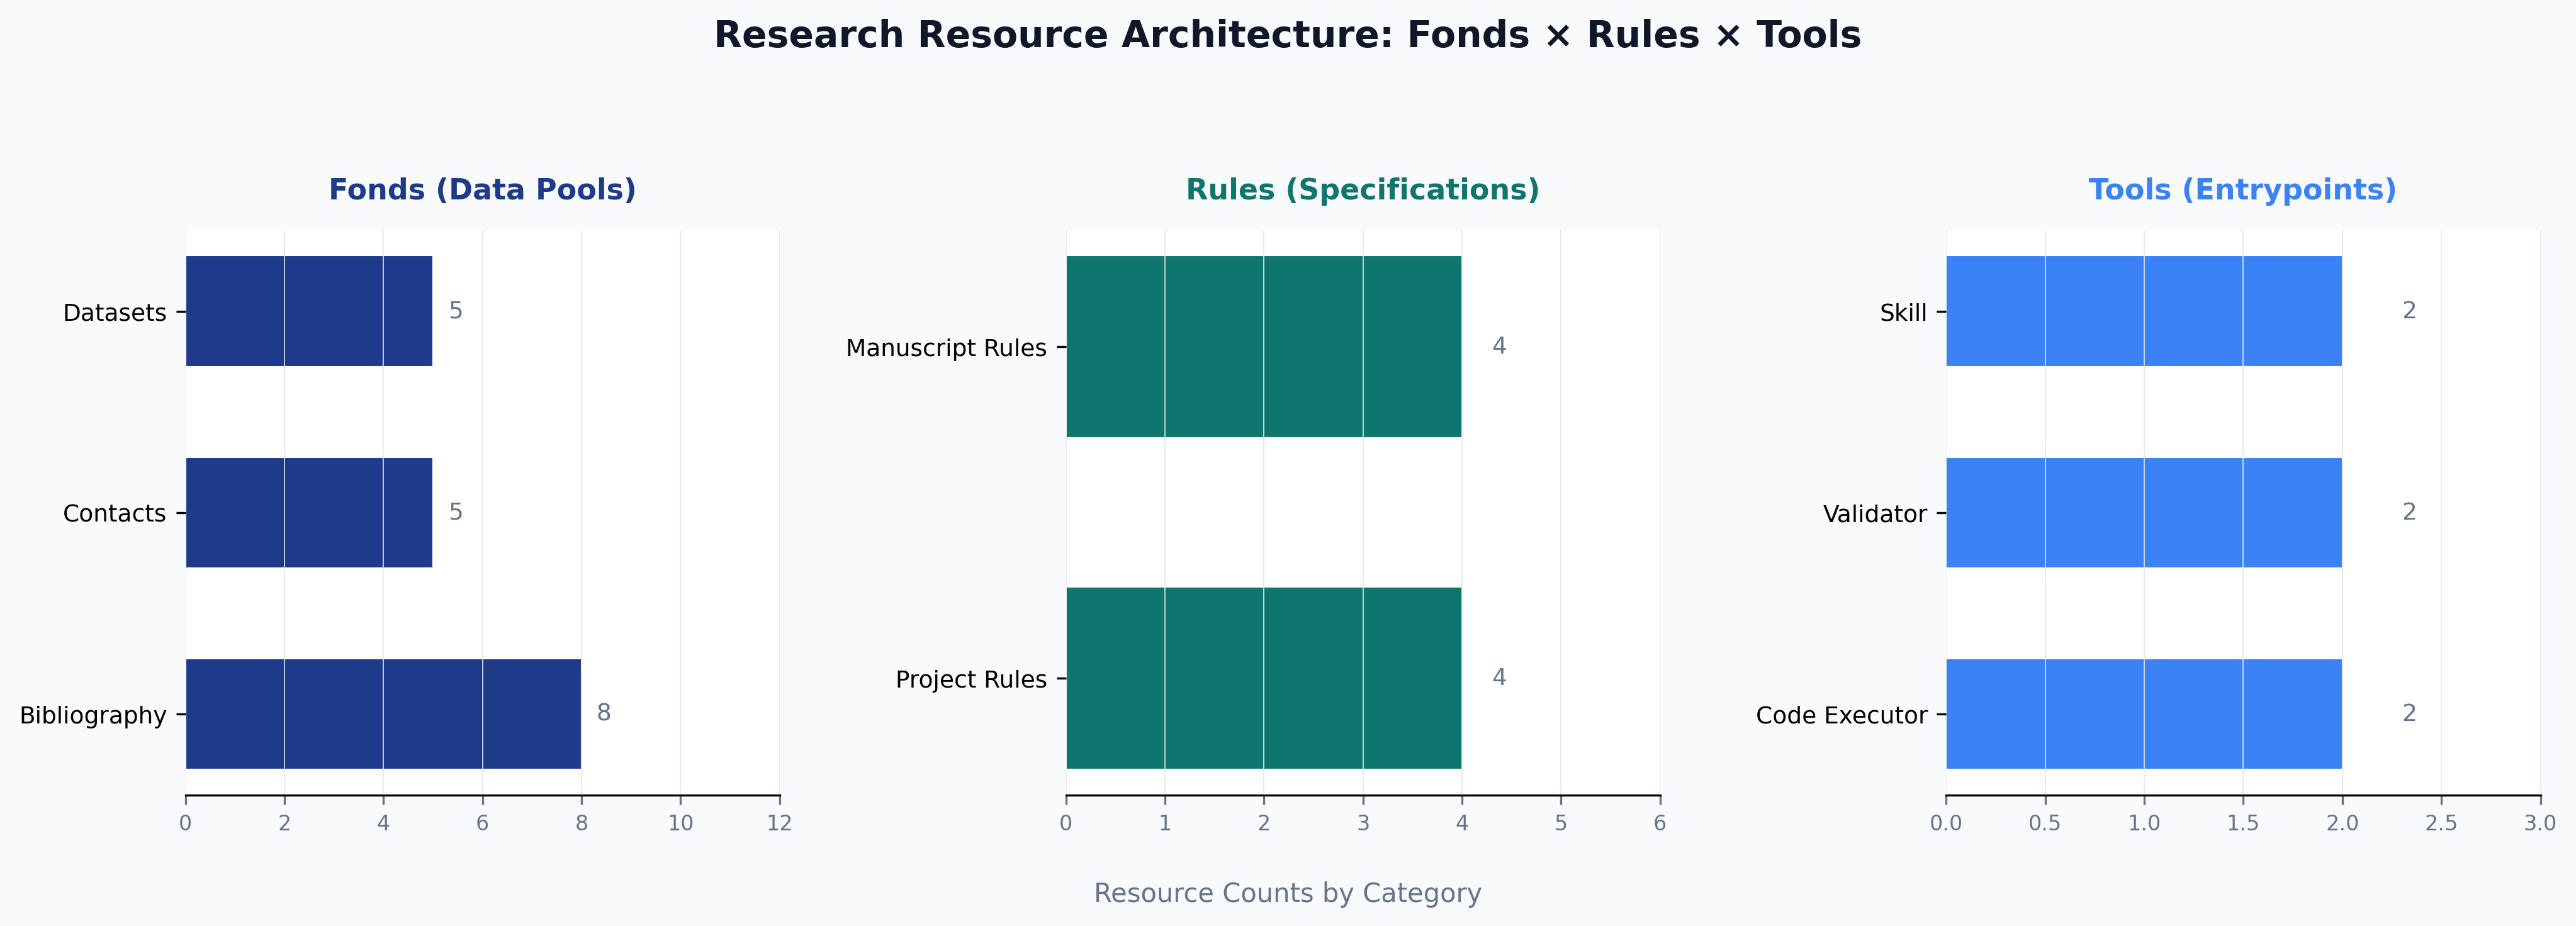
\includegraphics[width=0.9\linewidth,height=0.50\textheight,keepaspectratio,alt={Three-layer resource architecture of template\_pools\_rules\_tools. Fonds (left) provide read-only data pools; Rules (centre) provide governance constraints; Tools (right) provide executable entry points. The Integration layer (bottom) orchestrates all three.}]{../figures/architecture_overview.png}
\caption{Three-layer resource architecture of
template\_pools\_rules\_tools. Fonds (left) provide read-only data
pools; Rules (centre) provide governance constraints; Tools (right)
provide executable entry points. The Integration layer (bottom)
orchestrates all three.}\label{fig:architecture}
\end{figure}

The architecture obeys three design invariants:

\begin{itemize}
\tightlist
\item
  \textbf{Read-only resource access}: no module writes to
  \texttt{fonds/}, \texttt{rules/}, or \texttt{tools/}. The Layer
  Contract in \texttt{AGENTS.md} enforces this at code-review time.
\item
  \textbf{Repo-root-relative discovery}: all path resolution uses
  \texttt{pathlib.Path(\_\_file\_\_).resolve().parents{[}N{]}} so that
  scripts work from any working directory.
\item
  \textbf{Graceful degradation}: every reader checks file existence
  before parsing and catches \texttt{yaml.YAMLError} around the parse
  itself, logging a warning and returning a safe empty value either way.
  The pipeline never raises on a missing or malformed resource.
\end{itemize}

\subsection{Related Work and Alternative
Designs}\label{related-work-and-alternative-designs}

Three broad alternatives to the fonds/rules/tools pattern are common in
research-software monorepos, and each has a known failure mode this
design deliberately avoids.

\textbf{Shared library packages.} A monorepo could publish its
bibliography, contacts, and datasets as an installable Python package
(\breaktt{pip\ install\ monorepo-shared-data}) rather than a filesystem
convention. This works well for stable, versioned data but reintroduces
a packaging and release cycle for data that changes far more often than
code --- every bibliography update would require a version bump and a
re-install across every consuming project, which is precisely the
coordination overhead a monorepo is meant to eliminate.

\textbf{Symlink-based sharing.} Projects could symlink directly into a
shared resource directory rather than discovering it at runtime through
a reader module. This avoids the reader module's implementation cost but
loses the schema-validation and graceful-degradation layers: a symlinked
file that is malformed YAML fails wherever it is read, with no
structured \texttt{status} the pipeline can act on, and no compatibility
check against the manifest's \texttt{version} field.

\textbf{Environment-variable configuration.} Resource locations could be
injected via environment variables (\texttt{FONDS\_ROOT},
\texttt{RULES\_ROOT}) rather than resolved relative to the repository
root. This is the standard twelve-factor-app pattern for services, but
it is a poor fit for a forkable template repository: a contributor who
clones the repository and runs a script expects it to work without any
environment setup, and environment variables are precisely the kind of
implicit, undocumented dependency that a public exemplar should not
require.

The manifest-and-reader pattern adopted here --- versioned typed
manifests, repo-root-relative discovery, and graceful degradation ---
sits between these alternatives: no packaging overhead, structured
validation, and zero required environment configuration.
fig.~\ref{fig:pipelineflow} shows how this pattern integrates into the
project's script pipeline end-to-end.

\subsection{Paper Organisation}\label{paper-organisation}

The remainder of this paper is structured as follows.
sec.~\ref{sec:pools} describes the fond layer and the
\texttt{fonds\_reader} module, including the fond schema taxonomy
(fig.~\ref{fig:taxonomy}). sec.~\ref{sec:rules} describes the rules
layer and the \texttt{rules\_applier} module, including the soft/strong
rule hierarchy (fig.~\ref{fig:rulehier}). sec.~\ref{sec:tools} describes
the tool layer and the \texttt{tools\_invoker} module, including the
tool invocation contract (fig.~\ref{fig:toolcontract}).
sec.~\ref{sec:integration} presents the unified integration pipeline,
the manuscript variable token system, the three-level resilience design
(fig.~\ref{fig:resilience}), and the script pipeline
(fig.~\ref{fig:pipelineflow}). sec.~\ref{sec:conclusion} summarises key
findings, limitations, and future directions.

The architecture overview in fig.~\ref{fig:architecture} provides a
visual map of these relationships. Runtime statistics collected during
integration are visualised in fig.~\ref{fig:counts}, and the
corresponding per-component pass/partial/missing states are shown in
fig.~\ref{fig:pipeline}.

\newpage

\section{Pools: Fonds as Passive Data Resources}\label{sec:pools}

\subsection{What Is a Fond?}\label{what-is-a-fond}

A \textbf{fond} is a versioned, read-only data pool that any project in
the repository can consume without modifying. The term evokes the
culinary concept of a concentrated stock --- a stable base that enriches
whatever is built on top of it. Fonds live under the top-level
\texttt{fonds/\textless{}scope\textgreater{}/\textless{}name\textgreater{}/}
directory, each containing a manifest file (\texttt{fonds.yaml}), a
\texttt{data/} subdirectory, and optional documentation. This
architecture separates \emph{data ownership} from \emph{data usage}:
research projects in \texttt{projects/} are consumers, not producers, of
fond data. The separation prevents the accretion of project-specific
mutations in shared resources --- a recurring source of reproducibility
failures in collaborative research software \citep{Wilson2014best}.

The three-layer taxonomy (bibliography, contacts, datasets) maps to the
three most common categories of curated research data: citable
literature, human collaboration networks, and input/output datasets.
Each category carries its own schema enforced by
\breaktt{rules/templates/template\_manuscript\_rules}.
fig.~\ref{fig:taxonomy} compares the three fond types field-by-field:
every fond shares a manifest and a \texttt{type} discriminator, but the
source-of-truth format, secondary mirror, and deduplication key differ
by category --- a consequence of each category's data having a naturally
different canonical representation (BibTeX for citations, YAML for
structured contact records, YAML for dataset metadata).

\begin{figure}
\centering
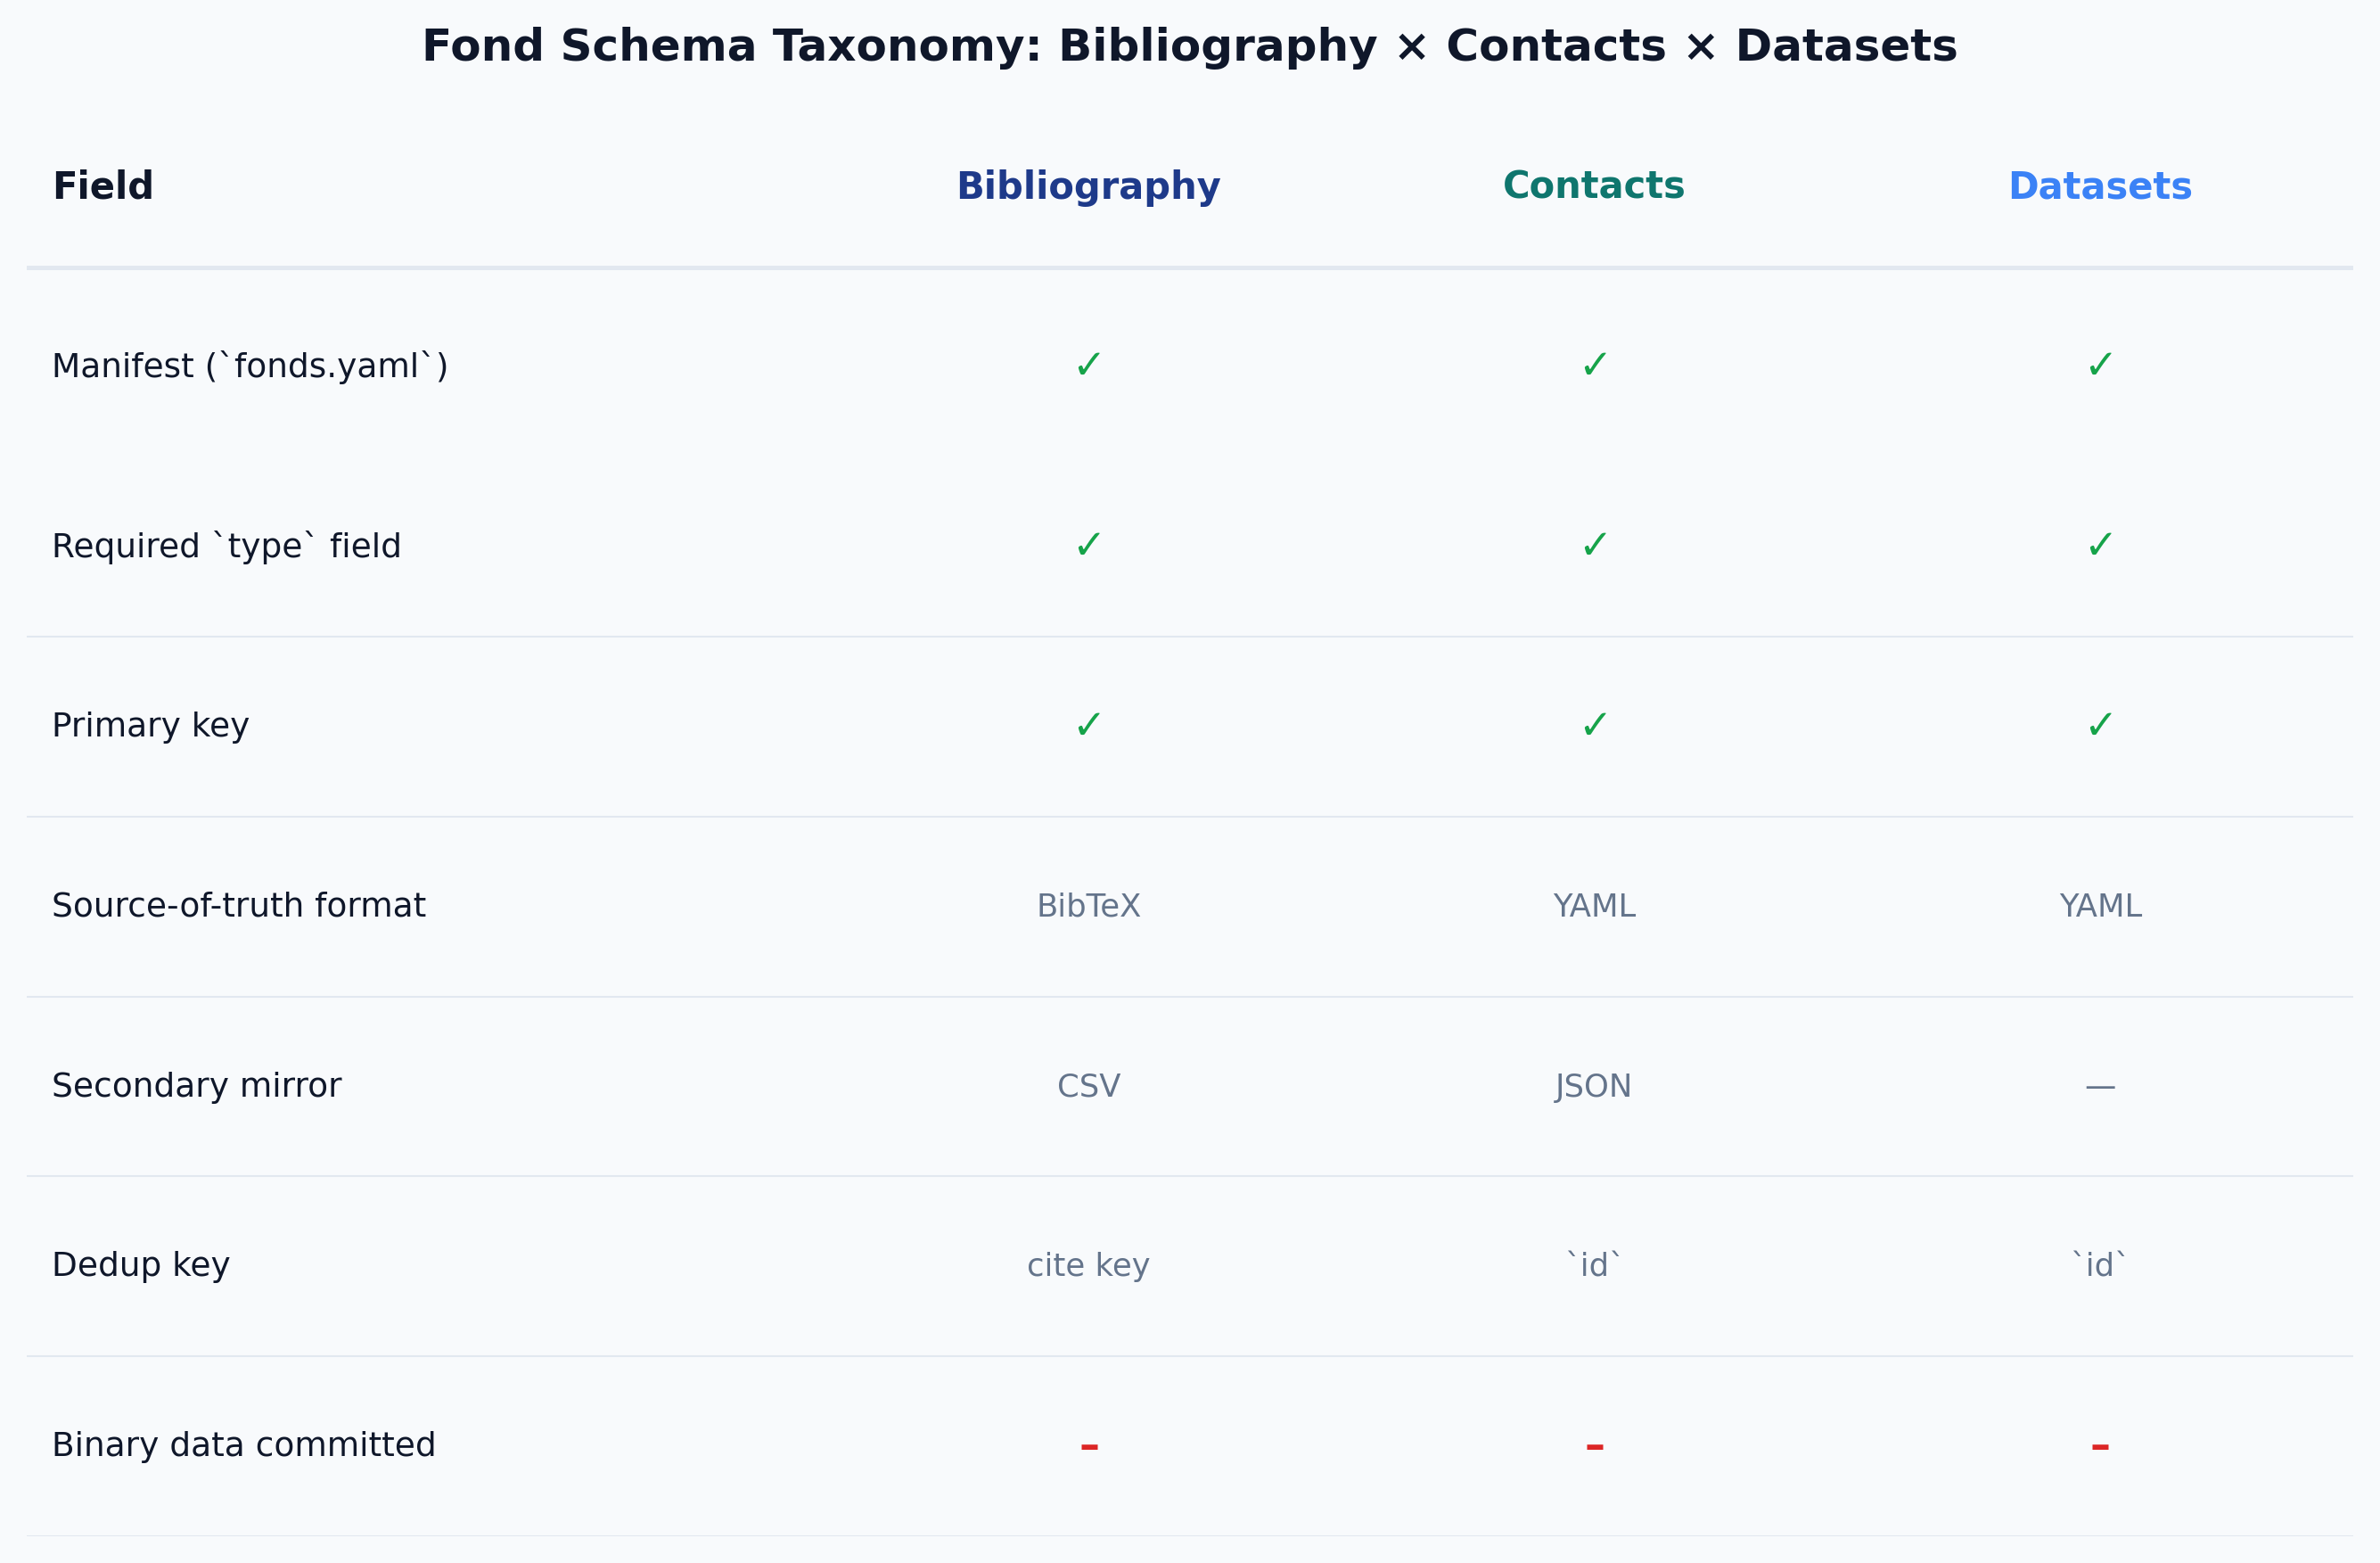
\includegraphics[width=0.85\linewidth,height=0.50\textheight,keepaspectratio,alt={Schema taxonomy comparison across the three fond types. Each fond declares a manifest and a type field; source-of-truth format, secondary mirror, and dedup key differ by category.}]{../figures/fond_taxonomy.png}
\caption{Schema taxonomy comparison across the three fond types. Each
fond declares a manifest and a \protect\texttt{type} field;
source-of-truth format, secondary mirror, and dedup key differ by
category.}\label{fig:taxonomy}
\end{figure}

\subsection{The Three Template Fonds}\label{the-three-template-fonds}

\subsubsection{\texorpdfstring{\breaktt{template\_bibliography}}{template_bibliography}}\label{template_bibliography}

The \breaktt{template\_bibliography} fond is a curated reference library
stored in two formats: a BibTeX file (\breaktt{data/references.bib}) as
source of truth, and a flat CSV export (\breaktt{data/references.csv})
for programmatic querying. Deduplication is enforced on the cite key
(the primary CSV column). The collection spans foundational
machine-learning works --- the transformer architecture
\citep{Vaswani2017attention}, early convolutional network research
\citep{LeCun1998gradient}, and large-scale language model pre-training
\citep{Brown2020gpt3} --- alongside software-engineering references on
best practices \citep{Wilson2014best} and robust software design
\citep{Taschuk2017ten}. In the current integration run, the fond
contains \textbf{8 entries}.

The bibliography fond illustrates the \emph{registry pattern}
\citep{Fowler2002patterns}: a single authoritative list is maintained
centrally, and all projects reference it rather than keeping private
copies. This guarantees citation consistency across all exemplar
manuscripts.

\subsubsection{\texorpdfstring{\breaktt{template\_contacts}}{template_contacts}}\label{template_contacts}

The \breaktt{template\_contacts} fond holds a registry of research
collaborators, advisors, and reviewers. Each entry is a YAML object with
required fields \texttt{id} (a unique slug), \texttt{name}, and
\texttt{email}, plus optional fields \texttt{affiliation},
\texttt{role}, \texttt{orcid}, \texttt{website}, and \texttt{notes}. The
YAML file (\breaktt{data/contacts.yaml}) is the source of truth; a JSON
mirror (\breaktt{data/contacts.json}) supports consumers that prefer JSON
deserialization. Deduplication is enforced on the \texttt{id} field at
validation time.

\subsubsection{\texorpdfstring{\breaktt{template\_datasets}}{template_datasets}}\label{template_datasets}

The \breaktt{template\_datasets} fond catalogs dataset metadata:
provenance, licensing, format, size, access URLs, and research tasks. It
intentionally stores \emph{metadata only} --- no actual data binaries
are committed to the repository. This design aligns with the principle
that version control systems should track configuration and metadata
rather than large binary artefacts \citep{Kluyver2016jupyter}. Dataset
entries require \texttt{id}, \texttt{name}, \texttt{version}, and
\texttt{license} fields. Exemplar entries reference classic benchmarks
such as MNIST (introduced in \citep{LeCun1998gradient}) and large-scale
corpora used in language-model research \citep{Brown2020gpt3}.

\subsection{\texorpdfstring{The \texttt{fonds.yaml}
Manifest}{The fonds.yaml Manifest}}\label{the-fonds.yaml-manifest}

Every fond root must contain a \texttt{fonds.yaml} manifest with at
minimum three fields:

\begin{Shaded}
\begin{Highlighting}[]
\FunctionTok{type}\KeywordTok{:}\AttributeTok{ bibliography}\CommentTok{   \# bibliography | contacts | datasets}
\FunctionTok{description}\KeywordTok{:}\AttributeTok{ }\StringTok{"Human{-}readable description of the fond"}
\FunctionTok{version}\KeywordTok{:}\AttributeTok{ }\StringTok{"1.0"}
\FunctionTok{tags}\KeywordTok{:}\AttributeTok{ }\KeywordTok{[}\AttributeTok{curated}\KeywordTok{,}\AttributeTok{ exemplar}\KeywordTok{]}
\end{Highlighting}
\end{Shaded}

The \texttt{type} field governs which reader function is appropriate and
what schema the \texttt{data/} directory is expected to follow. The
\texttt{version} field is incremented whenever the schema changes,
enabling consumers to detect and handle schema drift without silent
failures.

\subsection{\texorpdfstring{The \texttt{fonds\_reader}
Module}{The fonds_reader Module}}\label{the-fonds_reader-module}

The \breaktt{src/fonds\_reader.py} module provides three reader functions
--- one per fond type --- plus a convenience aggregator:

\begin{Shaded}
\begin{Highlighting}[]
\ImportTok{from}\NormalTok{ src.fonds\_reader }\ImportTok{import}\NormalTok{ (}
\NormalTok{    read\_bibliography\_fond,}
\NormalTok{    read\_contacts\_fond,}
\NormalTok{    read\_datasets\_fond,}
\NormalTok{    read\_all\_fonds,}
\NormalTok{)}

\NormalTok{bib      }\OperatorTok{=}\NormalTok{ read\_bibliography\_fond()   }\CommentTok{\# dict | None}
\NormalTok{contacts }\OperatorTok{=}\NormalTok{ read\_contacts\_fond()       }\CommentTok{\# dict | None}
\NormalTok{datasets }\OperatorTok{=}\NormalTok{ read\_datasets\_fond()       }\CommentTok{\# dict | None}
\NormalTok{all\_fonds }\OperatorTok{=}\NormalTok{ read\_all\_fonds()          }\CommentTok{\# \{"bibliography": ..., "contacts": ..., "datasets": ...\}}
\end{Highlighting}
\end{Shaded}

Each reader resolves the repository root from
\texttt{pathlib.Path(\_\_file\_\_).resolve().parents{[}4{]}}, checks
that the manifest and data files exist before touching them, and wraps
the actual YAML parse in a
\breaktt{try/except\ (OSError,\ UnicodeDecodeError,\ yaml.YAMLError)}
block. A missing path or a malformed file both degrade the same way ---
a logged warning and a \texttt{None} return --- so the integration
pipeline keeps going when a fond has not yet been populated by a
parallel agent \citep{Taschuk2017ten}. In the current run, 3 of 3
expected fonds were successfully loaded (see fig.~\ref{fig:counts}).

\subsection{Resilience by Design}\label{resilience-by-design}

The fond layer enforces resilience at two levels. At the
\textbf{structural} level, readers tolerate missing fonds entirely. At
the \textbf{schema} level, the manifest version field allows consumers
to check compatibility before processing data. This two-level approach
means a fond can evolve its schema without breaking existing consumers
that have not yet been updated: the consumer detects the version
mismatch and either adapts to it or skips the fond outright, instead of
crashing on data it doesn't recognise.

\subsection{Worked Example: Graceful Degradation in
Practice}\label{worked-example-graceful-degradation-in-practice}

Consider a concrete failure scenario: a parallel automation agent is in
the process of authoring \breaktt{fonds/templates/template\_contacts/}
and has written \texttt{fonds.yaml} but not yet populated
\breaktt{data/contacts.yaml}. A naive reader would raise
\breaktt{FileNotFoundError} the instant \breaktt{read\_contacts\_fond()}
is called, aborting the entire integration pipeline over one incomplete
resource. \breaktt{read\_contacts\_fond()} instead:

\begin{enumerate}
\def\labelenumi{\arabic{enumi}.}
\tightlist
\item
  Resolves the repository root via
  \texttt{pathlib.Path(\_\_file\_\_).resolve().parents{[}4{]}}.
\item
  Checks \breaktt{manifest\_path.exists()} and
  \breaktt{contacts\_path.exists()} explicitly before any read; on a
  missing path, logs
  \breaktt{logger.warning("contacts\ fond:\ missing\ \%s",\ p)} and
  returns \texttt{None} immediately --- no exception is ever raised for
  the common case of an in-progress resource.
\item
  If both paths exist, parses each with \breaktt{yaml.safe\_load()}
  inside a
  \breaktt{try/except\ (OSError,\ UnicodeDecodeError,\ yaml.YAMLError)}
  block, so a present-but-malformed file degrades the same way as a
  missing one.
\item
  \breaktt{run\_integration\_demo()} records the reduced count in the
  summary dict rather than propagating any exception.
\item
  The manuscript token \texttt{3} reflects the reduced count honestly
  --- the pipeline never claims a fond loaded that did not.
\end{enumerate}

This sequence is exercised directly by
\breaktt{tests/test\_fonds\_reader.py::test\_missing\_data\_dir\_contacts\_returns\_none},
which constructs a fond directory with a manifest but no \texttt{data/}
subdirectory and asserts the reader returns \texttt{None} rather than
raising. The same existence-check-then-parse pattern repeats identically
across \texttt{fonds\_reader.py}'s three readers,
\breaktt{rules\_applier.py}, and \breaktt{tools\_invoker.py}, which is why
fig.~\ref{fig:resilience} presents it as one repeated design, not three
independent ad-hoc fixes.

\newpage

\section{Rules: Soft and Strong Governance}\label{sec:rules}

\subsection{The Role of Governance
Rules}\label{the-role-of-governance-rules}

Research software projects make dozens of implicit governance decisions:
what test-coverage threshold is acceptable, how manuscript sections
should be ordered, which citation fields are mandatory. Left implicit,
these decisions drift silently across projects in a monorepo, eroding
the consistency that makes the repository valuable as a public exemplar.
The rules layer makes governance explicit, versioned, and
machine-enforceable.

A \textbf{rule set} in the template repository is a directory under
\texttt{rules/\textless{}scope\textgreater{}/\textless{}name\textgreater{}/}
containing a typed manifest (\texttt{rules.yaml}) and two subdirectories
of rule files:

\begin{verbatim}
<name>/
├── rules.yaml       — manifest (type, scope, version, rule_kinds)
├── soft/            — Markdown guideline files (human-readable, prompt-like)
└── strong/          — YAML constraint schemas (machine-enforceable)
\end{verbatim}

This two-tier architecture reflects the distinction between
\emph{guidance} (which humans follow approximately) and
\emph{constraints} (which pipelines enforce precisely) --- a distinction
also recognised in enterprise application architecture
\citep{Fowler2002patterns}. fig.~\ref{fig:rulehier} shows both template
rule sets split into their soft and strong branches: each branch is
independently discoverable, so a consumer that only cares about
machine-enforceable constraints never has to parse guideline prose, and
vice versa.

\subsection{Soft Rules: Style and Process
Guidelines}\label{soft-rules-style-and-process-guidelines}

Soft rules are Markdown files in \texttt{soft/}. They encode preferences
and conventions that cannot easily be expressed as boolean constraints
but that human reviewers and AI agents can apply contextually. Examples
include:

\begin{itemize}
\tightlist
\item
  \textbf{Style preferences}: ``Prefer active voice in manuscript
  sections.'' ``Use \texttt{\textbackslash{}module\{\}} macros for all
  code identifiers.''
\item
  \textbf{Process guidelines}: ``Tag pull requests with a review-stage
  label before requesting review.'' ``Update \texttt{TODO.md} before
  closing an issue.''
\item
  \textbf{Citation conventions}: ``Cite primary sources rather than
  textbooks where possible.''
\end{itemize}

Soft rules are treated as guidance: deviations surface as suggestions in
code review and manuscript audit reports, not as pipeline blockers. This
makes the soft layer suitable for evolving preferences that should not
break automated checks.

\subsection{Strong Rules: Hard
Constraints}\label{strong-rules-hard-constraints}

Strong rules are YAML files in \texttt{strong/}. Each file defines one
named constraint:

\begin{Shaded}
\begin{Highlighting}[]
\FunctionTok{rule}\KeywordTok{:}
\AttributeTok{  }\FunctionTok{name}\KeywordTok{:}\AttributeTok{ coverage{-}gate}
\AttributeTok{  }\FunctionTok{kind}\KeywordTok{:}\AttributeTok{ strong}
\AttributeTok{  }\FunctionTok{description}\KeywordTok{:}\AttributeTok{ }\StringTok{"Minimum test coverage threshold for src/ modules."}
\AttributeTok{  }\FunctionTok{applies\_to}\KeywordTok{:}\AttributeTok{ }\StringTok{"projects/*/src/"}
\AttributeTok{  }\FunctionTok{enforcement}\KeywordTok{:}\AttributeTok{ fail\_on\_violation}
\AttributeTok{  }\FunctionTok{constraints}\KeywordTok{:}
\AttributeTok{    }\FunctionTok{minimum\_line\_coverage}\KeywordTok{:}\AttributeTok{ }\DecValTok{90}
\AttributeTok{    }\FunctionTok{minimum\_branch\_coverage}\KeywordTok{:}\AttributeTok{ }\DecValTok{80}
\end{Highlighting}
\end{Shaded}

The \breaktt{enforcement:\ fail\_on\_violation} field signals that a
pipeline must halt and report when this rule is violated. Strong rules
are suitable for invariants that, if broken, indicate a genuine defect
rather than a style preference: coverage below 90\% means tests are
missing; a manuscript section without an abstract means the document is
incomplete.

\begin{figure}
\centering
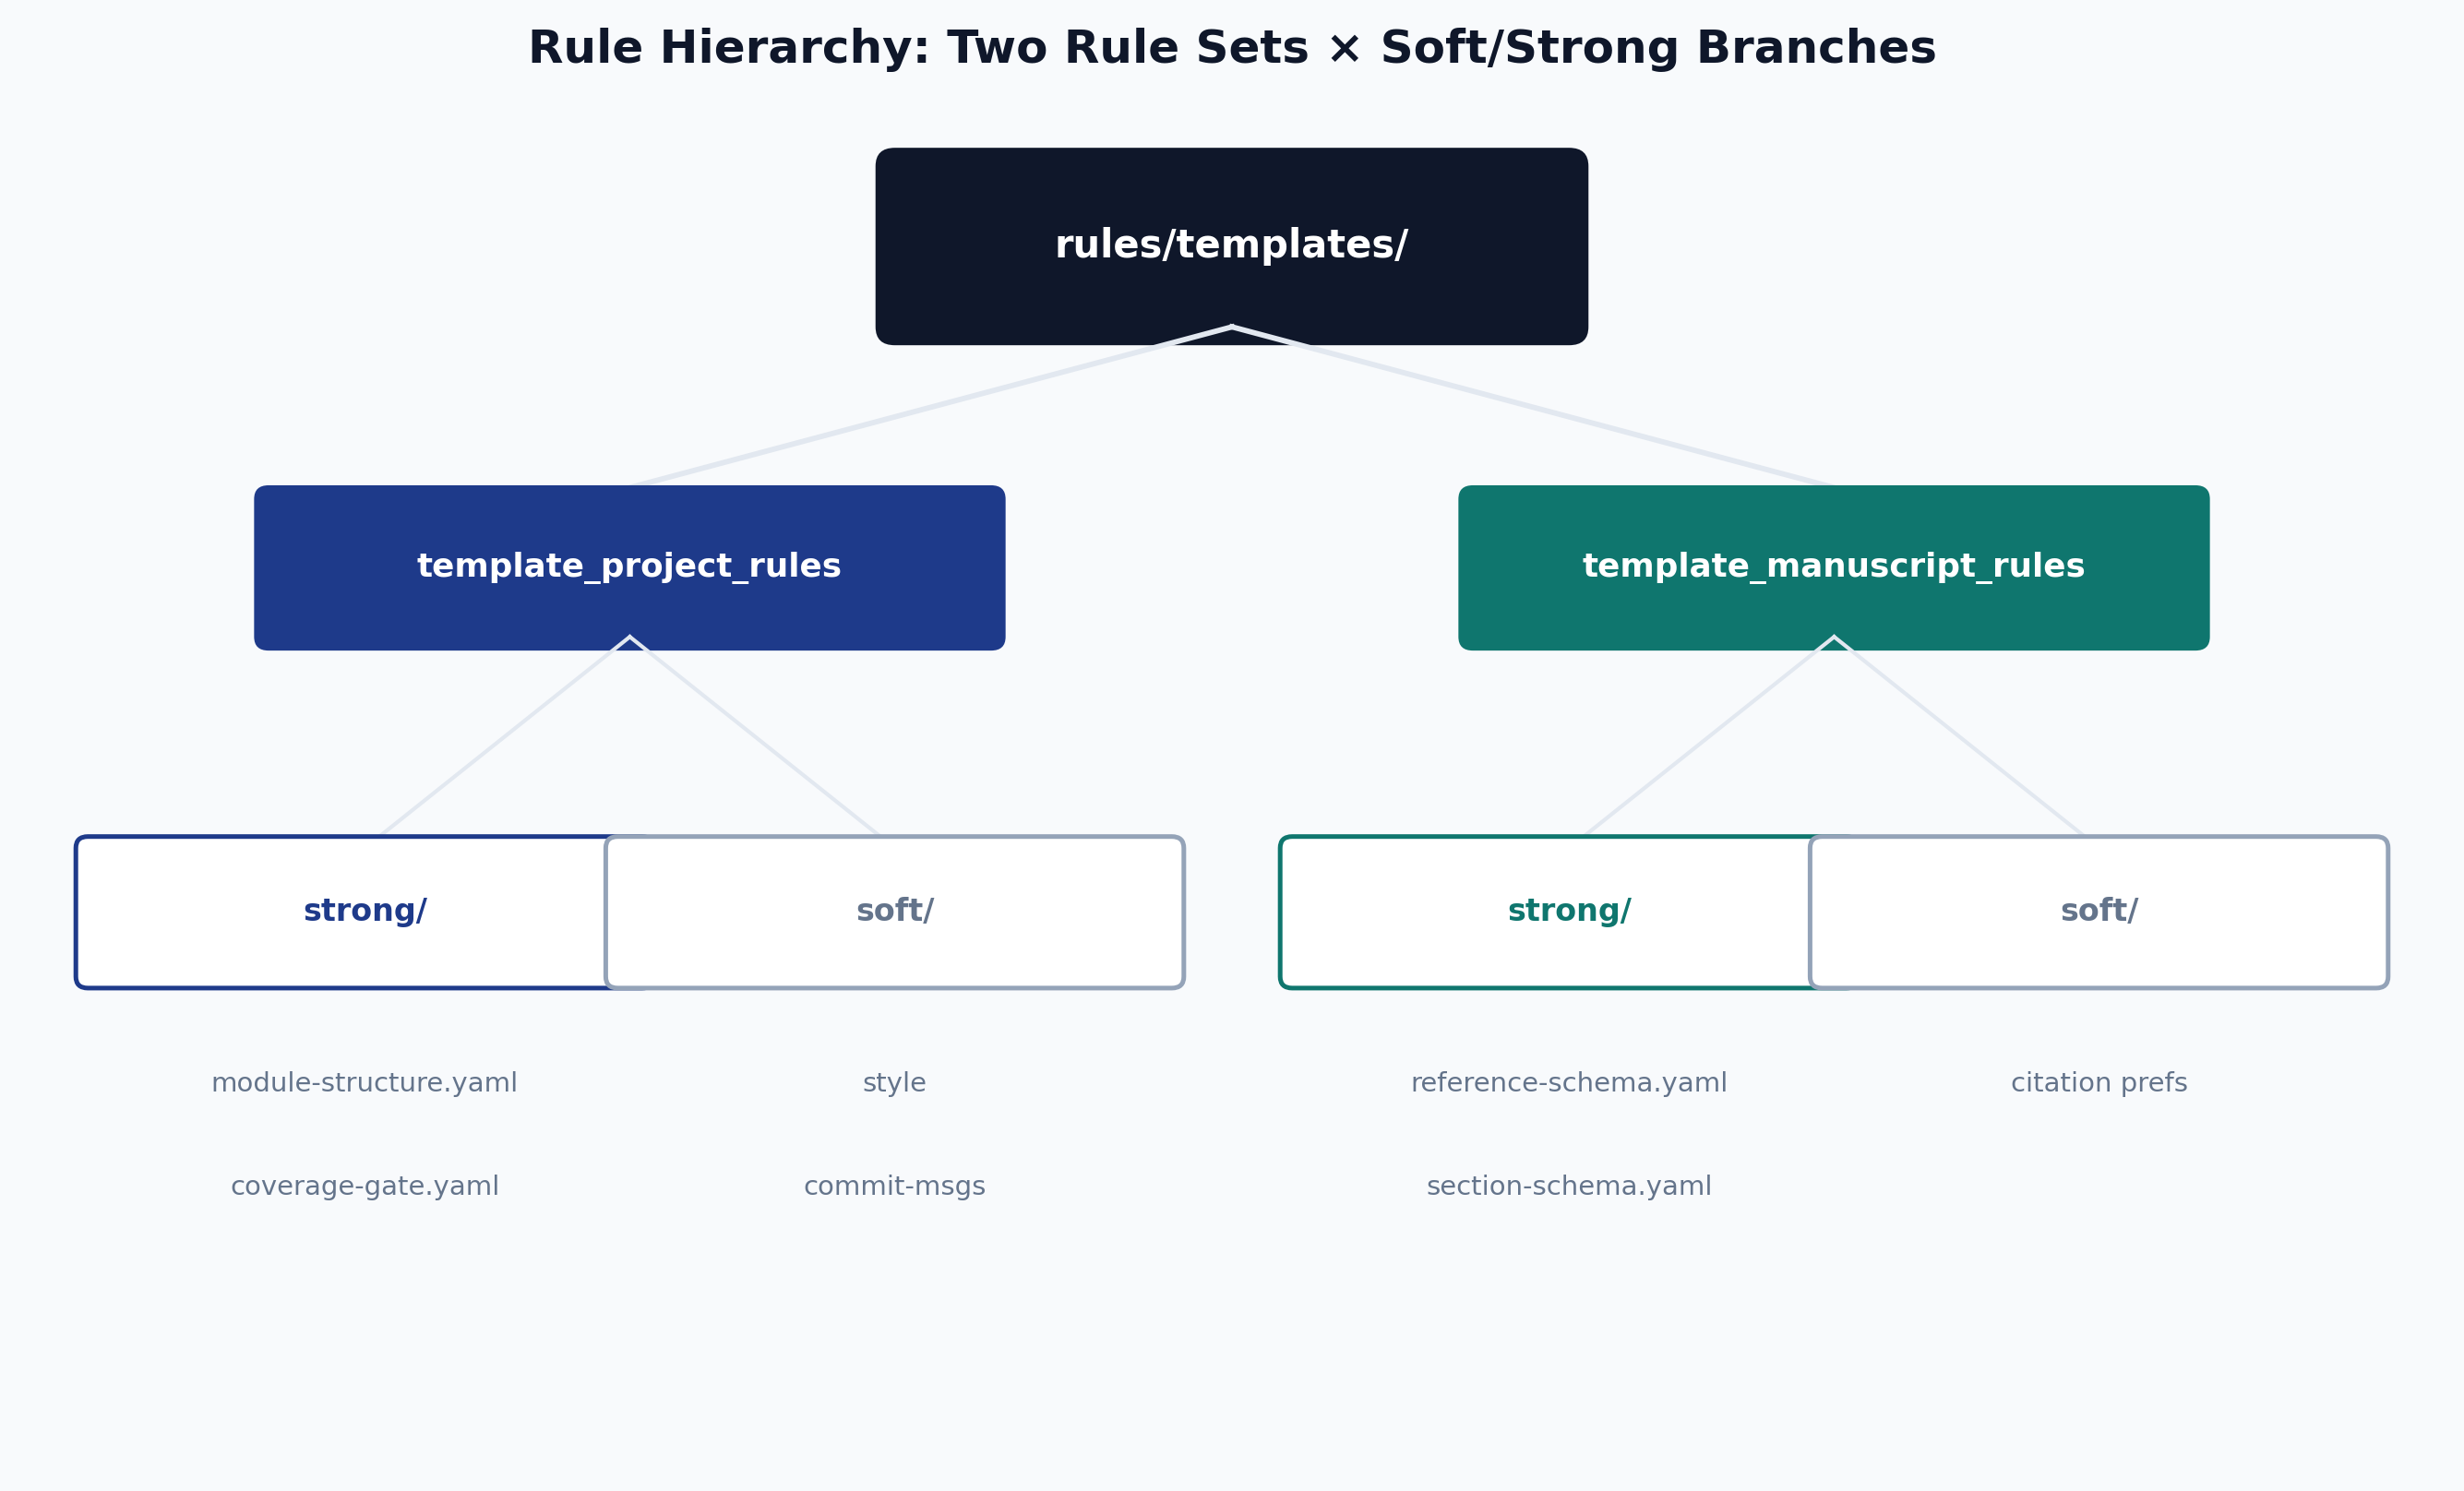
\includegraphics[width=0.85\linewidth,height=0.50\textheight,keepaspectratio,alt={Rule hierarchy: the two template rule sets, each split into a machine-enforceable strong/ branch and a guidance-only soft/ branch.}]{../figures/rule_hierarchy.png}
\caption{Rule hierarchy: the two template rule sets, each split into a
machine-enforceable \protect\texttt{strong/} branch and a guidance-only
\protect\texttt{soft/} branch.}\label{fig:rulehier}
\end{figure}

\subsection{The Two Template Rule
Sets}\label{the-two-template-rule-sets}

\subsubsection{\texorpdfstring{\breaktt{template\_project\_rules}}{template_project_rules}}\label{template_project_rules}

This rule set governs software projects throughout the template
repository. Its strong rules currently comprise:

{\def\LTcaptype{none} % do not increment counter
\begin{longtable}[]{@{}
  >{\raggedright\arraybackslash}p{(\linewidth - 2\tabcolsep) * \real{0.5000}}
  >{\raggedright\arraybackslash}p{(\linewidth - 2\tabcolsep) * \real{0.5000}}@{}}
\toprule\noalign{}
\begin{minipage}[b]{\linewidth}\raggedright
File
\end{minipage} & \begin{minipage}[b]{\linewidth}\raggedright
Constraint
\end{minipage} \\
\midrule\noalign{}
\endhead
\bottomrule\noalign{}
\endlastfoot
\breaktt{strong/coverage-gate.yaml} & Minimum line coverage 90\%, branch
coverage 80\% for \texttt{src/} \\
\breaktt{strong/module-structure.yaml} & Required directory layout:
\texttt{src/}, \texttt{tests/}, \texttt{scripts/},
\texttt{manuscript/} \\
\end{longtable}
}

Its soft rules provide guidance on code style, commit message
conventions, and pull-request labelling.

\subsubsection{\texorpdfstring{\breaktt{template\_manuscript\_rules}}{template_manuscript_rules}}\label{template_manuscript_rules}

This rule set governs research manuscripts. Its strong rules comprise:

{\def\LTcaptype{none} % do not increment counter
\begin{longtable}[]{@{}
  >{\raggedright\arraybackslash}p{(\linewidth - 2\tabcolsep) * \real{0.5000}}
  >{\raggedright\arraybackslash}p{(\linewidth - 2\tabcolsep) * \real{0.5000}}@{}}
\toprule\noalign{}
\begin{minipage}[b]{\linewidth}\raggedright
File
\end{minipage} & \begin{minipage}[b]{\linewidth}\raggedright
Constraint
\end{minipage} \\
\midrule\noalign{}
\endhead
\bottomrule\noalign{}
\endlastfoot
\breaktt{strong/reference-schema.yaml} & Required BibTeX fields and
cite-key format constraints \\
\breaktt{strong/section-schema.yaml} & Required manuscript sections,
ordering, and minimum word counts \\
\end{longtable}
}

In the current pipeline run, \textbf{2 of 2 rule sets} validated
successfully (fig.~\ref{fig:counts}).

\subsection{\texorpdfstring{The \texttt{rules\_applier}
Module}{The rules_applier Module}}\label{the-rules_applier-module}

The \breaktt{src/rules\_applier.py} module exposes three functions:

\begin{Shaded}
\begin{Highlighting}[]
\ImportTok{from}\NormalTok{ src.rules\_applier }\ImportTok{import}\NormalTok{ (}
\NormalTok{    load\_soft\_rules,}
\NormalTok{    load\_strong\_rules,}
\NormalTok{    validate\_against\_rules,}
\NormalTok{)}

\NormalTok{soft   }\OperatorTok{=}\NormalTok{ load\_soft\_rules(}\StringTok{"template\_project\_rules"}\NormalTok{)    }\CommentTok{\# list[dict]}
\NormalTok{strong }\OperatorTok{=}\NormalTok{ load\_strong\_rules(}\StringTok{"template\_project\_rules"}\NormalTok{)  }\CommentTok{\# list[dict]}
\NormalTok{result }\OperatorTok{=}\NormalTok{ validate\_against\_rules(}\StringTok{"template\_project\_rules"}\NormalTok{)}
\CommentTok{\# → \{"status": "ok" | "partial" | "missing", "soft\_count": N, "strong\_count": N\}}
\end{Highlighting}
\end{Shaded}

\breaktt{validate\_against\_rules()} performs two checks: (1) the
\texttt{rules.yaml} manifest is parseable YAML; (2) every rule file in
\texttt{soft/} and \texttt{strong/} is parseable YAML. It returns a
status of \texttt{"ok"} when both checks pass, \texttt{"partial"} when
the manifest exists but some rule files are missing or malformed, and
\texttt{"missing"} when the rule set directory is absent entirely. This
graduated status enables the integration pipeline to distinguish between
a rule set that has not yet been created (acceptable during active
development) and one that is present but broken (actionable defect).

\subsection{Rules and Manuscript
Variables}\label{rules-and-manuscript-variables}

Strong rule validation counts are injected into the manuscript through
the token system. The token \texttt{2} expands to the count of rule sets
that returned \texttt{status="ok"} during the integration run. This
creates a verifiable link between the pipeline's actual behaviour and
the manuscript's claims --- the manuscript cannot assert successful
validation without the pipeline having actually succeeded.

\subsection{\texorpdfstring{Beyond Structural Validation: The
\breaktt{strong\_rule\_evaluator}
Module}{Beyond Structural Validation: The strong_rule_evaluator Module}}\label{beyond-structural-validation-the-strong_rule_evaluator-module}

\breaktt{validate\_against\_rules()} (described above) performs
\emph{structural} validation only: it confirms that \texttt{rules.yaml}
and every file in \texttt{soft/}/\texttt{strong/} parse as YAML. It does
not check whether the constraints those strong-rule files declare are
actually satisfied by the current project. That semantic layer lives in
a separate module, \breaktt{src/strong\_rule\_evaluator.py}, exposed via
\breaktt{scripts/04\_validate\_strong\_rules.py}:

\begin{Shaded}
\begin{Highlighting}[]
\ImportTok{from}\NormalTok{ src.strong\_rule\_evaluator }\ImportTok{import}\NormalTok{ evaluate\_strong\_rules, load\_rule\_context\_from\_project}

\NormalTok{context }\OperatorTok{=}\NormalTok{ load\_rule\_context\_from\_project(project\_root)}
\NormalTok{result }\OperatorTok{=}\NormalTok{ evaluate\_strong\_rules(}\StringTok{"template\_project\_rules"}\NormalTok{, context)}
\CommentTok{\# → \{"rule\_set": ..., "evaluations": [...], "passed": bool, "violation\_count": int\}}
\end{Highlighting}
\end{Shaded}

\breaktt{evaluate\_strong\_rules()} dispatches each strong-rule YAML file
to a rule-kind-specific evaluator function keyed by its declared kind,
via a small dispatch table covering all four strong-rule kinds that
exist across both rule sets:

{\def\LTcaptype{none} % do not increment counter
\begin{longtable}[]{@{}
  >{\raggedright\arraybackslash}p{(\linewidth - 4\tabcolsep) * \real{0.3333}}
  >{\raggedright\arraybackslash}p{(\linewidth - 4\tabcolsep) * \real{0.3333}}
  >{\raggedright\arraybackslash}p{(\linewidth - 4\tabcolsep) * \real{0.3333}}@{}}
\toprule\noalign{}
\begin{minipage}[b]{\linewidth}\raggedright
Kind
\end{minipage} & \begin{minipage}[b]{\linewidth}\raggedright
Evaluator
\end{minipage} & \begin{minipage}[b]{\linewidth}\raggedright
Checks
\end{minipage} \\
\midrule\noalign{}
\endhead
\bottomrule\noalign{}
\endlastfoot
\breaktt{coverage\_threshold} & \breaktt{\_evaluate\_coverage\_threshold}
& Measured coverage percentages (from \texttt{context{[}"coverage"{]}})
against each constraint's declared \breaktt{minimum\_line\_coverage} \\
\breaktt{module\_structure} & \breaktt{\_evaluate\_module\_structure} &
Required project directory layout (\texttt{src/}, \texttt{tests/},
\texttt{scripts/}, \texttt{manuscript/}) actually exists \\
\texttt{section\_schema} & \breaktt{\_evaluate\_section\_schema} &
Required manuscript sections, ordering, and forbidden placeholder
headings (\texttt{TODO}, \texttt{Draft}, etc.) \\
\breaktt{reference\_schema} & \breaktt{\_evaluate\_reference\_schema} &
Required BibTeX fields and cite-key format constraints on every parsed
reference entry \\
\end{longtable}
}

Each evaluator distinguishes structured violation \emph{reasons} rather
than collapsing everything to a boolean --- for example,
\breaktt{coverage\_threshold} reports separately whether a key was absent
from context (a context-completeness issue), non-numeric (a
context-shape issue), or numeric-but-below-minimum (a genuine rule
violation). This is what lets the pipeline tell a maintainer \emph{why}
a rule failed, not merely \emph{that} it failed --- directly addressing
the ``actionable defect'' distinction introduced in the previous
section.

Crucially, \texttt{section\_schema} and \breaktt{reference\_schema} are
not evaluated against synthetic fixtures ---
\breaktt{load\_rule\_context\_from\_project()} (in
\breaktt{scripts/04\_validate\_strong\_rules.py}) builds their context by
parsing \emph{this project's own, current}
\breaktt{manuscript/references.bib} into structured reference entries and
extracting the real \texttt{\#}-level headings from every file under
\texttt{manuscript/*.md}. Running
\breaktt{uv\ run\ python\ projects/templates/template\_pools\_rules\_tools/scripts/04\_validate\_strong\_rules.py}
therefore semantically validates this exact manuscript's own
bibliography and section structure, live, on every invocation --- re-run
that command to see the current evaluation and violation counts rather
than trusting a number printed here, since either count can legitimately
change as the manuscript grows.

\newpage

\section{Tools: Executable Entry Points}\label{sec:tools}

\subsection{What Is a Tool?}\label{what-is-a-tool}

A \textbf{tool} in the template repository is a directory under
\texttt{tools/\textless{}scope\textgreater{}/\textless{}name\textgreater{}/}
that packages one or more executable scripts behind a typed manifest
(\texttt{tools.yaml}). Tools provide the third layer of the resource
architecture: where fonds supply static data and rules supply governance
constraints, tools supply \emph{behaviour} --- computations, validation
runs, and agent skill invocations that projects can trigger without
re-implementing the underlying logic.

The tools layer deliberately mirrors the Unix philosophy of small,
composable utilities that communicate through standard interfaces
\citep{Raymond2003art}. Each tool declares its entrypoints (shell
scripts), its invocation contract (stdin/stdout/exit-code semantics),
and its capabilities (type, version, tags) in a single manifest file.
Consumers invoke tools through the \texttt{tools\_invoker} module
without needing to understand the tool's implementation details --- a
textbook application of the Facade pattern \citep{Gamma1994design}.

\subsection{\texorpdfstring{The \texttt{tools.yaml}
Manifest}{The tools.yaml Manifest}}\label{the-tools.yaml-manifest}

Every tool root must contain a \texttt{tools.yaml} manifest with the
following fields:

\begin{Shaded}
\begin{Highlighting}[]
\FunctionTok{type}\KeywordTok{:}\AttributeTok{ code\_executor | validator | skill | agent | renderer}
\FunctionTok{description}\KeywordTok{:}\AttributeTok{ }\StringTok{"Human{-}readable description of the tool"}
\FunctionTok{version}\KeywordTok{:}\AttributeTok{ }\StringTok{"1.0.0"}
\FunctionTok{tags}\KeywordTok{:}\AttributeTok{ }\KeywordTok{[}\AttributeTok{curated}\KeywordTok{,}\AttributeTok{ exemplar}\KeywordTok{,}\AttributeTok{ production}\KeywordTok{,}\AttributeTok{ experimental}\KeywordTok{]}
\FunctionTok{creator}\KeywordTok{:}\AttributeTok{ }\StringTok{"org/repo"}
\FunctionTok{license}\KeywordTok{:}\AttributeTok{ }\StringTok{"Apache{-}2.0"}
\FunctionTok{entrypoints}\KeywordTok{:}
\AttributeTok{  }\KeywordTok{{-}}\AttributeTok{ scripts/run.sh}
\AttributeTok{  }\KeywordTok{{-}}\AttributeTok{ scripts/validate.sh}
\end{Highlighting}
\end{Shaded}

The \texttt{type} field determines the invocation contract the consumer
should expect. The \texttt{entrypoints} list names the scripts that must
exist on disk; the \texttt{tools\_invoker} module validates their
presence at discovery time rather than at invocation time, making
failures visible early in the pipeline rather than at runtime.
fig.~\ref{fig:toolcontract} visualises the stdin/stdout/exit-code
contract for all three template tools side by side; note that the
\emph{shape} of stdin and stdout differs per tool while the
\emph{presence} of a well-defined contract does not --- this is what
makes \texttt{tools\_invoker} able to discover and validate any tool
generically without knowing its payload schema.

\begin{figure}
\centering
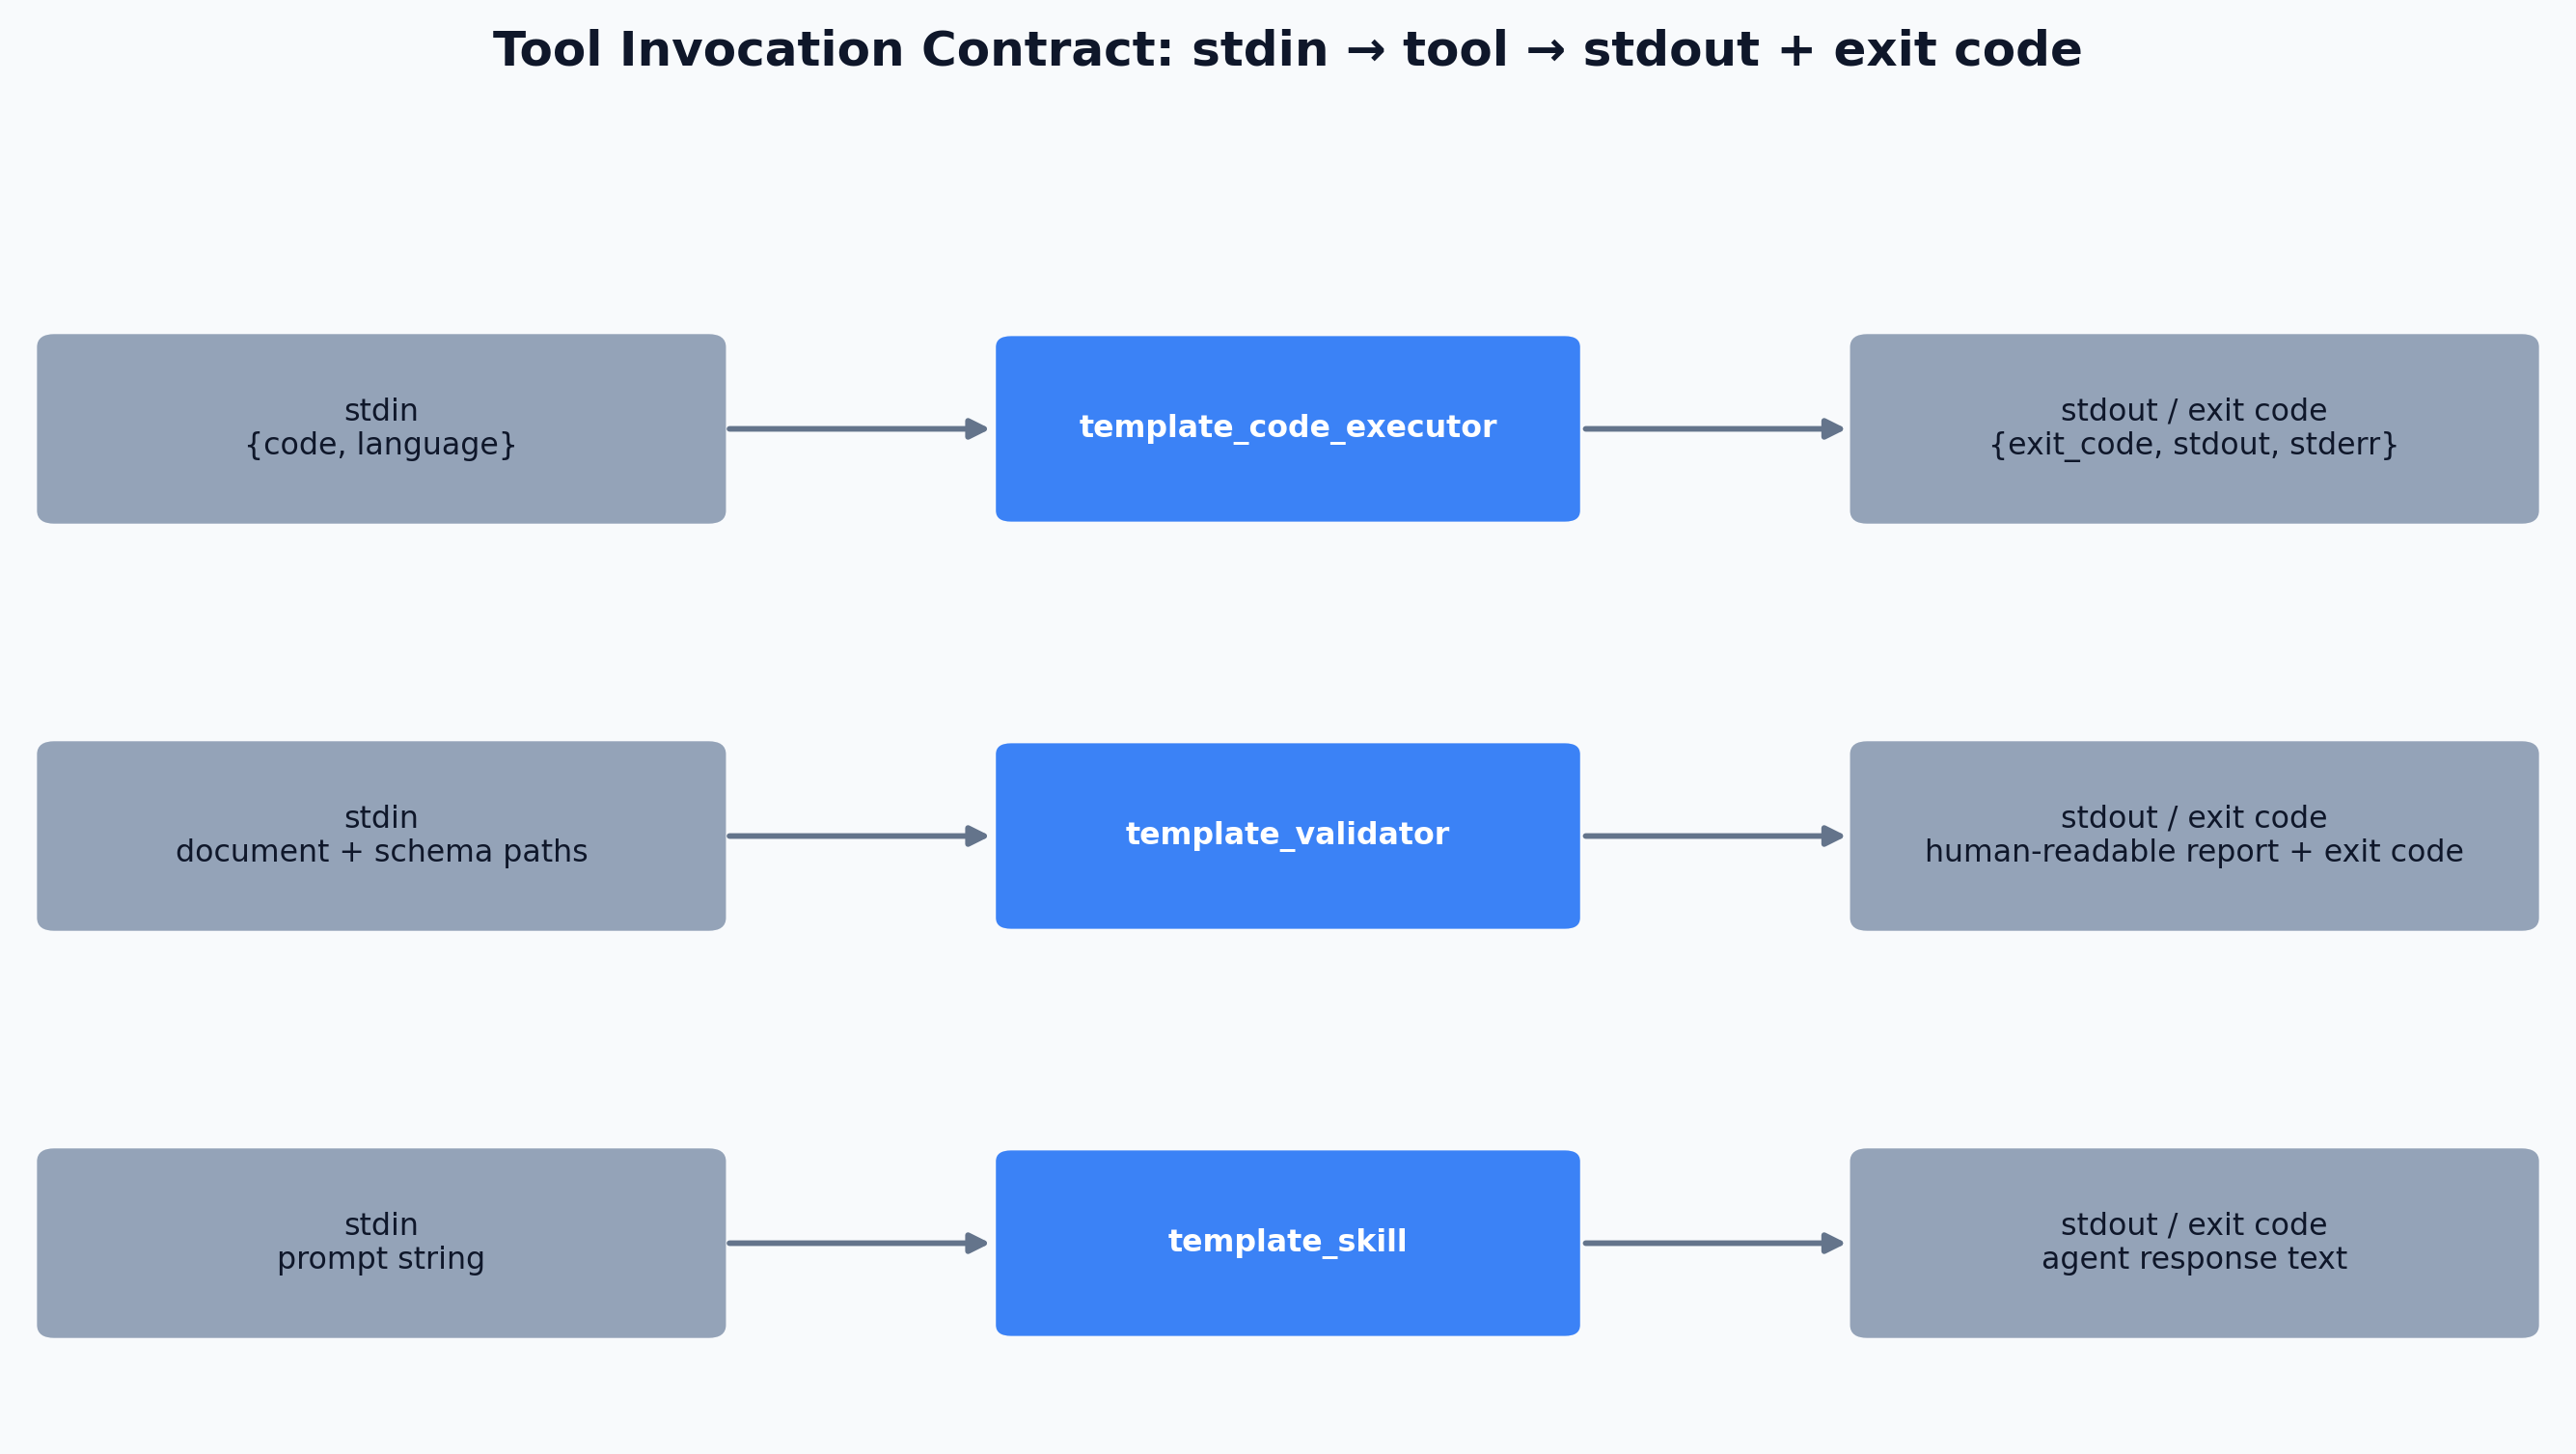
\includegraphics[width=0.9\linewidth,height=0.50\textheight,keepaspectratio,alt={Invocation contract for the three template tools: stdin payload, tool behaviour, and stdout/exit-code shape.}]{../figures/tool_contract.png}
\caption{Invocation contract for the three template tools: stdin
payload, tool behaviour, and stdout/exit-code
shape.}\label{fig:toolcontract}
\end{figure}

\subsection{The Three Template Tools}\label{the-three-template-tools}

\subsubsection{\texorpdfstring{\breaktt{template\_code\_executor}}{template_code_executor}}\label{template_code_executor}

A generic code execution tool that accepts a JSON payload on standard
input and returns execution results as JSON. The invocation contract is:

{\def\LTcaptype{none} % do not increment counter
\begin{longtable}[]{@{}
  >{\raggedright\arraybackslash}p{(\linewidth - 6\tabcolsep) * \real{0.2500}}
  >{\raggedright\arraybackslash}p{(\linewidth - 6\tabcolsep) * \real{0.2500}}
  >{\raggedright\arraybackslash}p{(\linewidth - 6\tabcolsep) * \real{0.2500}}
  >{\raggedright\arraybackslash}p{(\linewidth - 6\tabcolsep) * \real{0.2500}}@{}}
\toprule\noalign{}
\begin{minipage}[b]{\linewidth}\raggedright
Entrypoint
\end{minipage} & \begin{minipage}[b]{\linewidth}\raggedright
stdin
\end{minipage} & \begin{minipage}[b]{\linewidth}\raggedright
stdout
\end{minipage} & \begin{minipage}[b]{\linewidth}\raggedright
exit code
\end{minipage} \\
\midrule\noalign{}
\endhead
\bottomrule\noalign{}
\endlastfoot
\texttt{scripts/run.sh} & \texttt{\{"code":\ str,\ "language":\ str\}} &
\texttt{\{"exit\_code":\ int,\ "stdout":\ str,\ "stderr":\ str\}} & 0 =
success \\
\breaktt{scripts/validate.sh} & --- & Human-readable validation report &
0 = valid \\
\end{longtable}
}

The code executor exemplifies tools that wrap a computational
capability. The JSON-in/JSON-out contract makes it easily composable
with pipeline orchestrators and agent frameworks.

\subsubsection{\texorpdfstring{\breaktt{template\_validator}}{template_validator}}\label{template_validator}

A JSON Schema validation tool. It reads a target document and a schema
from disk and reports validation results in human-readable form. The
entrypoint \breaktt{scripts/validate.sh} exits 0 when the document is
valid and non-zero with a detailed error message otherwise. The
validator tool is used in the project pipeline to validate
\breaktt{manuscript\_variables.json} against its expected schema before
manuscript rendering.

\subsubsection{\texorpdfstring{\texttt{template\_skill}}{template_skill}}\label{template_skill}

An agent skill invocation tool that wraps a Hermes-compatible skill
definition. The entrypoint \breaktt{scripts/invoke.sh} accepts a prompt
string on standard input and returns the agent response as text. This
tool type bridges the repository's tool architecture with external agent
frameworks, demonstrating that the same manifest-and-entrypoint pattern
applies equally to computational tools and AI agents.

Unlike the two tools above, \breaktt{scripts/invoke.sh} requires a real
\texttt{OPENAI\_API\_KEY} and makes a paid network call to
\texttt{api.openai.com} --- it is therefore never invoked by this
project's tests or pipeline, by design. Offline reproducibility is a
stated requirement of this exemplar (see the front-matter
Reproducibility Checklist), and no CI job in this repository injects
\texttt{OPENAI\_API\_KEY} into this project's test run.
\breaktt{template\_code\_executor} and \breaktt{template\_validator}, by
contrast, are fully local and deterministic --- see the Execution-Proof
Testing subsection below for how this project actually exercises them.

\subsection{\texorpdfstring{The \texttt{tools\_invoker}
Module}{The tools_invoker Module}}\label{the-tools_invoker-module}

The \breaktt{src/tools\_invoker.py} module provides three public
functions:

\begin{Shaded}
\begin{Highlighting}[]
\ImportTok{from}\NormalTok{ src.tools\_invoker }\ImportTok{import}\NormalTok{ (}
\NormalTok{    discover\_tools,}
\NormalTok{    get\_tool\_entrypoints,}
\NormalTok{    validate\_tool\_scripts\_exist,}
\NormalTok{)}

\NormalTok{tools }\OperatorTok{=}\NormalTok{ discover\_tools()}
\CommentTok{\# → [\{"name": "template\_code\_executor", "manifest": \{...\}\}, ...]}

\NormalTok{eps }\OperatorTok{=}\NormalTok{ get\_tool\_entrypoints(}\StringTok{"template\_code\_executor"}\NormalTok{)}
\CommentTok{\# → ["scripts/run.sh", "scripts/validate.sh"]}

\NormalTok{result }\OperatorTok{=}\NormalTok{ validate\_tool\_scripts\_exist(}\StringTok{"template\_code\_executor"}\NormalTok{)}
\CommentTok{\# → \{"status": "ok" | "partial" | "missing", "missing\_scripts": [...]\}}
\end{Highlighting}
\end{Shaded}

\breaktt{discover\_tools()} scans \breaktt{tools/templates/} and returns
one \texttt{ToolEntry} per subdirectory, regardless of whether a
manifest is present: a directory with a parseable \texttt{tools.yaml}
gets \texttt{manifest=\{...\}}; a directory with no manifest, or one
that fails to parse, gets \texttt{manifest=None} plus a logged warning.
Discovery itself never raises and never drops a directory from the
result --- the \emph{interpretation} of ``not a real tool yet'' is left
to the caller (\breaktt{get\_tool\_entrypoints()} and
\breaktt{validate\_tool\_scripts\_exist()} both return an
empty/\texttt{"missing"} result for a \texttt{None} manifest), which
keeps discovery and validation as separate, independently testable
concerns.

\breaktt{validate\_tool\_scripts\_exist()} iterates over the manifest's
\texttt{entrypoints} list and checks each path against the filesystem.
It returns a structured result distinguishing between tools that are
fully ready (\texttt{"ok"}), partially configured (\texttt{"partial"}
--- some scripts missing), and entirely absent (\texttt{"missing"}). In
the current integration run, \textbf{3 tools} were discovered
(fig.~\ref{fig:counts}), all with valid manifests.

\subsection{Tool Discovery and
Reproducibility}\label{tool-discovery-and-reproducibility}

The tools layer contributes to reproducibility by making the
\emph{availability} of computational capabilities explicit and
checkable. A project that hard-codes a path to a tool script becomes
brittle when the repository is reorganised. By contrast, a project that
calls \breaktt{discover\_tools()} and checks
\breaktt{validate\_tool\_scripts\_exist()} will detect missing
entrypoints at pipeline initialisation time and report them clearly,
rather than failing silently at execution time
\citep{Stodden2016enhancing}. This shift from implicit to explicit
dependency declaration is a key design principle of the template
architecture (see fig.~\ref{fig:architecture}).

\subsection{Tool Composition and Failure
Modes}\label{tool-composition-and-failure-modes}

Because every tool exposes the same discovery contract (manifest +
entrypoint list), tools compose without any consumer-side
special-casing. A pipeline stage that wants ``any validator'' can call
\breaktt{discover\_tools()}, filter the result list on
\texttt{manifest{[}"type"{]}\ ==\ "validator"}, and invoke whichever
\breaktt{template\_validator}-typed tool it finds --- without hard-coding
\breaktt{template\_validator} by name. This composability comes with
three failure modes that \texttt{tools\_invoker} handles explicitly
rather than leaving to the caller:

\begin{enumerate}
\def\labelenumi{\arabic{enumi}.}
\tightlist
\item
  \textbf{Manifest present, entrypoint missing.}
  \breaktt{discover\_tools()} finds a parseable \texttt{tools.yaml}
  declaring \texttt{scripts/run.sh}, but the file does not exist.
  \breaktt{validate\_tool\_scripts\_exist()} surfaces this as
  \breaktt{status="partial"} with the specific missing path in
  \texttt{missing\_scripts}, catching the defect at discovery time
  instead of waiting for a caller to try executing the script.
\item
  \textbf{Manifest missing entirely.} A directory under
  \breaktt{tools/templates/} exists but has no \texttt{tools.yaml}.
  \breaktt{discover\_tools()} still returns a \texttt{ToolEntry} for it
  (with \texttt{manifest=None}, so the caller can see it exists), but
  \breaktt{get\_tool\_entrypoints()} and
  \breaktt{validate\_tool\_scripts\_exist()} both treat a \texttt{None}
  manifest as ``not yet a tool,'' returning an empty collection or
  \texttt{"missing"} status without ever raising --- this matters for
  partially-scaffolded work-in-progress tool directories created by a
  parallel agent.
\item
  \textbf{Manifest malformed YAML.} The same graceful-degradation
  pattern from sec.~\ref{sec:pools} applies here: a parse error is
  caught and logged, and the offending tool is quietly excluded from the
  discovery result, leaving the pipeline free to continue with
  everything else it found.
\end{enumerate}

Each of these is a distinct, testable branch in
\breaktt{tests/test\_tools\_invoker.py}, and each maps to one row of the
resilience taxonomy in fig.~\ref{fig:resilience}.

\subsection{Execution-Proof Testing: Beyond Manifest
Checking}\label{execution-proof-testing-beyond-manifest-checking}

Everything described so far --- discovery, entrypoint-existence
validation, the three failure modes above --- is \emph{structural}: it
confirms a tool's files are present and well-formed without ever running
them. \breaktt{src/tools\_invoker.py}'s public API deliberately stays
that way, because subprocess execution is exactly the kind of operation
that can raise (a missing \texttt{bash}/\texttt{jq}/\texttt{python3}
binary, a permission error, a timeout), and this project's readers are
contracted to degrade gracefully rather than propagate exceptions (see
sec.~\ref{sec:pools}).

The test suite closes this gap without weakening that contract:
\breaktt{tests/test\_tools\_invoker.py} genuinely subprocess-invokes the
two fully local, deterministic tools and asserts on their real output,
rather than only checking that their scripts exist.

\begin{itemize}
\tightlist
\item
  \textbf{\breaktt{template\_code\_executor}}:
  \breaktt{TestInvokeCodeExecutor} pipes
  \texttt{\{"code":\ "print(2\ +\ 2)",\ "language":\ "python"\}} into
  the real \texttt{scripts/run.sh} and asserts the parsed JSON result
  has \breaktt{exit\_code\ ==\ 0} and \texttt{"4"} in \texttt{stdout} ---
  and, as a negative control, pipes code that calls
  \breaktt{raise\ SystemExit(3)} and asserts the real
  \breaktt{exit\_code\ ==\ 3} comes back.
\item
  \textbf{\breaktt{template\_validator}}: \breaktt{TestInvokeValidator}
  pipes a schema-conformant document into the real
  \breaktt{scripts/validate.sh} and asserts \breaktt{returncode\ ==\ 0}
  and \texttt{"VALID"} in stdout; a document missing the
  \texttt{version} field required by the tool's own \texttt{schema.json}
  is asserted to return \breaktt{returncode\ ==\ 1} and
  \texttt{"INVALID"} --- a genuine, schema-verified violation, not an
  assumed one.
\end{itemize}

Both test classes are guarded with \breaktt{pytest.mark.skipif} on the
real runtime dependency each script needs
(\texttt{timeout}/\texttt{gtimeout} plus \texttt{jq} for the code
executor; the \texttt{jsonschema} package for the validator), so a
missing binary skips the test cleanly instead of failing it --- on the
machine this manuscript was rendered on, the code-executor tests skip
(no \texttt{timeout}/\texttt{gtimeout} on this macOS host) while the
validator tests run for real, which is itself a demonstration of the
skip-guard working as intended rather than masking a failure.

\newpage

\section{Integration: Unified Pipeline and Token
Injection}\label{sec:integration}

\subsection{Architecture Overview}\label{architecture-overview}

The three resource layers described in sec.~\ref{sec:pools},
sec.~\ref{sec:rules}, and sec.~\ref{sec:tools} are orchestrated by a
single function in \breaktt{src/integration.py}. The
\breaktt{run\_integration\_demo()} function calls all three subsystems in
a defined order, collects their results into a structured dictionary,
and writes summary counts to
\breaktt{output/data/manuscript\_variables.json} for injection into this
manuscript at render time. fig.~\ref{fig:architecture} illustrates the
complete architecture.

\begin{verbatim}
run_integration_demo()
  ├── read_bibliography_fond()       → {"manifest": ..., "bibtex": ..., "csv_rows": [...]}
  ├── read_contacts_fond()           → {"manifest": ..., "contacts": [...]}
  ├── read_datasets_fond()           → {"manifest": ..., "datasets": [...]}
  ├── validate_against_rules("template_project_rules")    → {"status": "ok", ...}
  ├── validate_against_rules("template_manuscript_rules") → {"status": "ok", ...}
  ├── discover_tools()               → [{"name": ..., "manifest": ...}, ...]
  └── validate_tool_scripts_exist(<each tool>)            → {"status": "ok", ...}
\end{verbatim}

The function returns a top-level dict with keys \texttt{fonds},
\texttt{rules}, \texttt{tools}, and \texttt{summary}. The
\texttt{summary} sub-dict provides the counts that populate manuscript
tokens.

\subsection{Manuscript Variable
Tokens}\label{manuscript-variable-tokens}

The token injection system bridges the integration pipeline and the
manuscript prose. Tokens use double-brace syntax: \texttt{3} expands to
the integer count of fonds successfully loaded during the most recent
integration run. Tokens are resolved by
\breaktt{scripts/03\_generate\_manuscript.py}, which reads
\breaktt{output/data/manuscript\_variables.json} and substitutes each
token before the manuscript is passed to the rendering engine.

\begin{figure}
\centering
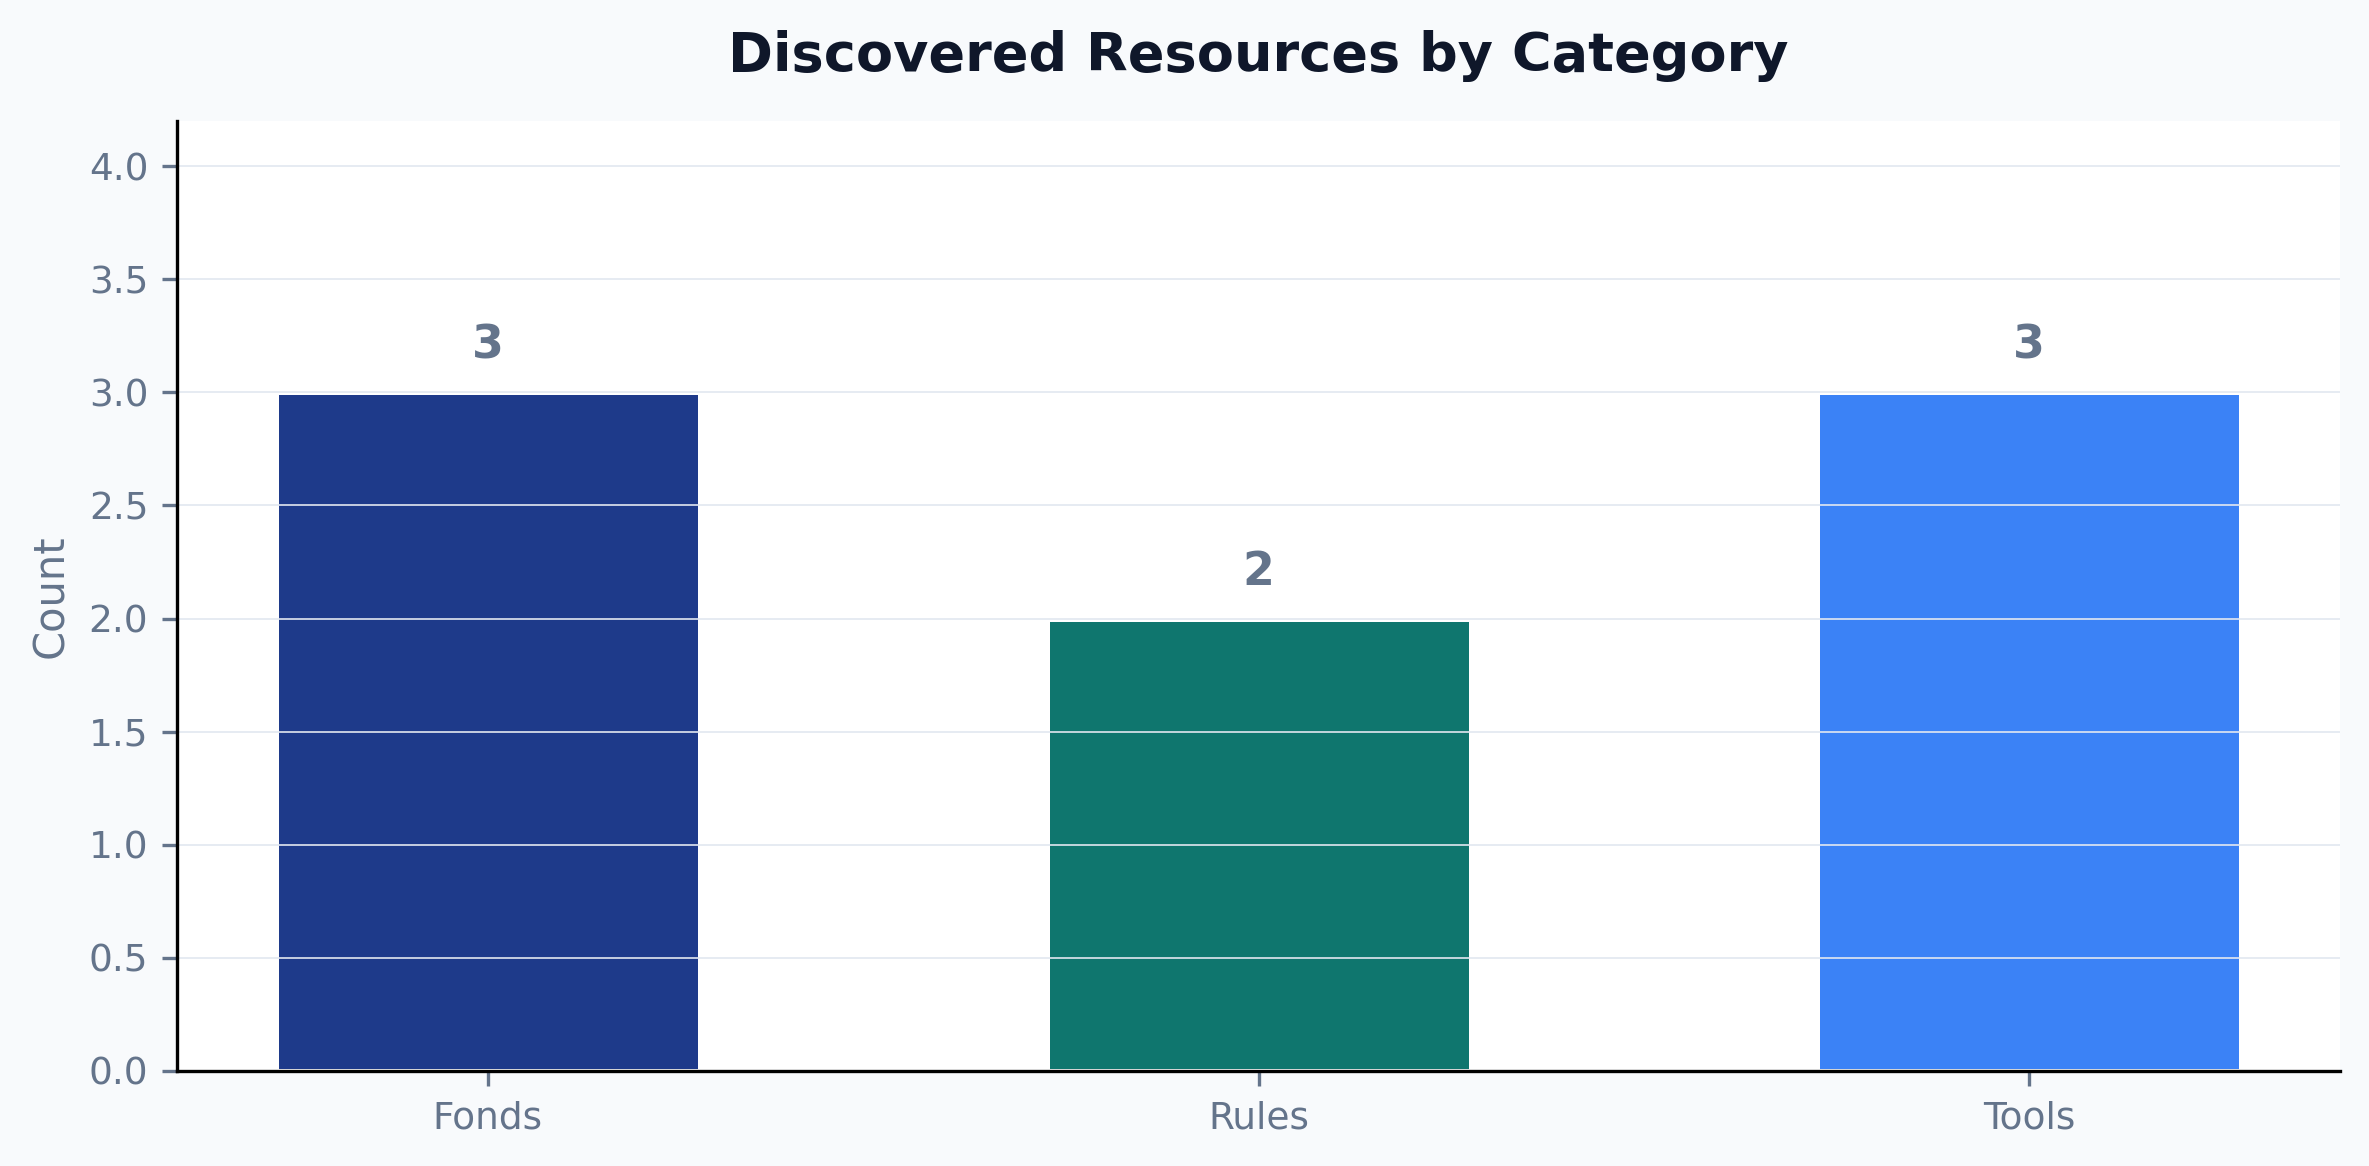
\includegraphics[width=0.75\linewidth,height=0.50\textheight,keepaspectratio,alt={Runtime integration counts from manuscript\_variables.json. Bars show fonds loaded, rule sets validated, and tools discovered during a single pipeline run.}]{../figures/resource_counts.png}
\caption{Runtime integration counts from manuscript\_variables.json.
Bars show fonds loaded, rule sets validated, and tools discovered during
a single pipeline run.}\label{fig:counts}
\end{figure}

The current \breaktt{manuscript\_variables.json} contains the following
summary values (see fig.~\ref{fig:counts} for a visual representation):

{\def\LTcaptype{none} % do not increment counter
\begin{longtable}[]{@{}ll@{}}
\toprule\noalign{}
Token & Value \\
\midrule\noalign{}
\endhead
\bottomrule\noalign{}
\endlastfoot
\texttt{3} & 3 \\
\texttt{2} & 2 \\
\texttt{3} & 3 \\
\texttt{8} & 8 \\
\end{longtable}
}

This table is itself token-injected: the values shown are those produced
by the pipeline, not hard-coded by the manuscript author. If the
pipeline results change --- for example, because a new fond is added ---
re-running \breaktt{scripts/03\_generate\_manuscript.py} updates the
manuscript automatically, without manual editing. This property is
central to reproducibility: the manuscript's quantitative claims are
always consistent with the code that generated them
\citep{Stodden2016enhancing}.

\subsection{Methods: The Script
Pipeline}\label{methods-the-script-pipeline}

Six thin orchestration scripts govern the integration workflow
(fig.~\ref{fig:pipeline}, fig.~\ref{fig:pipelineflow}):

{\def\LTcaptype{none} % do not increment counter
\begin{longtable}[]{@{}
  >{\raggedright\arraybackslash}p{(\linewidth - 4\tabcolsep) * \real{0.3333}}
  >{\raggedright\arraybackslash}p{(\linewidth - 4\tabcolsep) * \real{0.3333}}
  >{\raggedright\arraybackslash}p{(\linewidth - 4\tabcolsep) * \real{0.3333}}@{}}
\toprule\noalign{}
\begin{minipage}[b]{\linewidth}\raggedright
Script
\end{minipage} & \begin{minipage}[b]{\linewidth}\raggedright
Purpose
\end{minipage} & \begin{minipage}[b]{\linewidth}\raggedright
Key output
\end{minipage} \\
\midrule\noalign{}
\endhead
\bottomrule\noalign{}
\endlastfoot
\breaktt{scripts/01\_validate\_sources.py} & Validate presence and
well-formedness of all resources & Console report \\
\breaktt{scripts/02\_run\_integration.py} & Run
\breaktt{run\_integration\_demo()} and print JSON summary & Console
JSON \\
\breaktt{scripts/03\_generate\_manuscript.py} & Write
\breaktt{output/data/manuscript\_variables.json} & JSON file \\
\breaktt{scripts/04\_validate\_strong\_rules.py} & Semantic evaluation of
strong-rule constraints (sec.~\ref{sec:rules}) against this project's
own tree & Console report, non-zero exit on violation \\
\breaktt{scripts/05\_generate\_figures.py} & Render all 8 content figures
plus the cover illustration & 9 PNG files under
\breaktt{manuscript/figures/} \\
\breaktt{scripts/z\_generate\_manuscript\_variables.py} & Hydrate
\texttt{\{\{TOKEN\}\}} values and inject them into
\breaktt{output/manuscript/} immediately before rendering & JSON file +
resolved manuscript tree \\
\end{longtable}
}

\begin{figure}
\centering
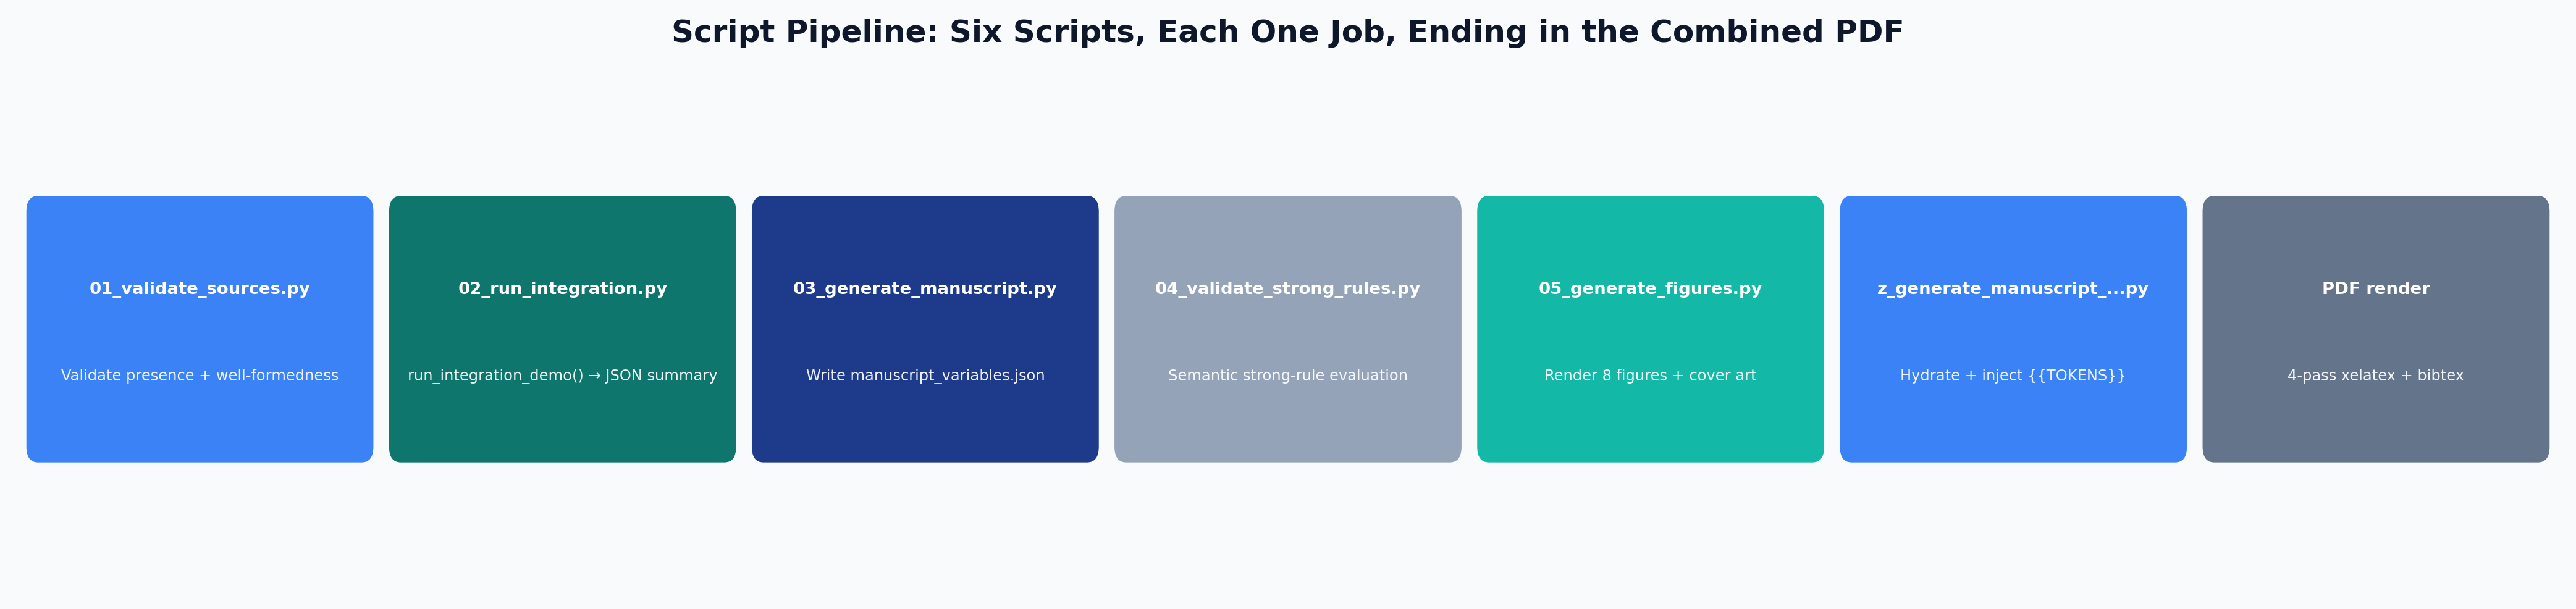
\includegraphics[width=0.95\linewidth,height=0.50\textheight,keepaspectratio,alt={The six-script pipeline from source validation through token hydration, ending at the combined-PDF render step.}]{../figures/pipeline_flow.png}
\caption{The six-script pipeline from source validation through token
hydration, ending at the combined-PDF render
step.}\label{fig:pipelineflow}
\end{figure}

\begin{figure}
\centering
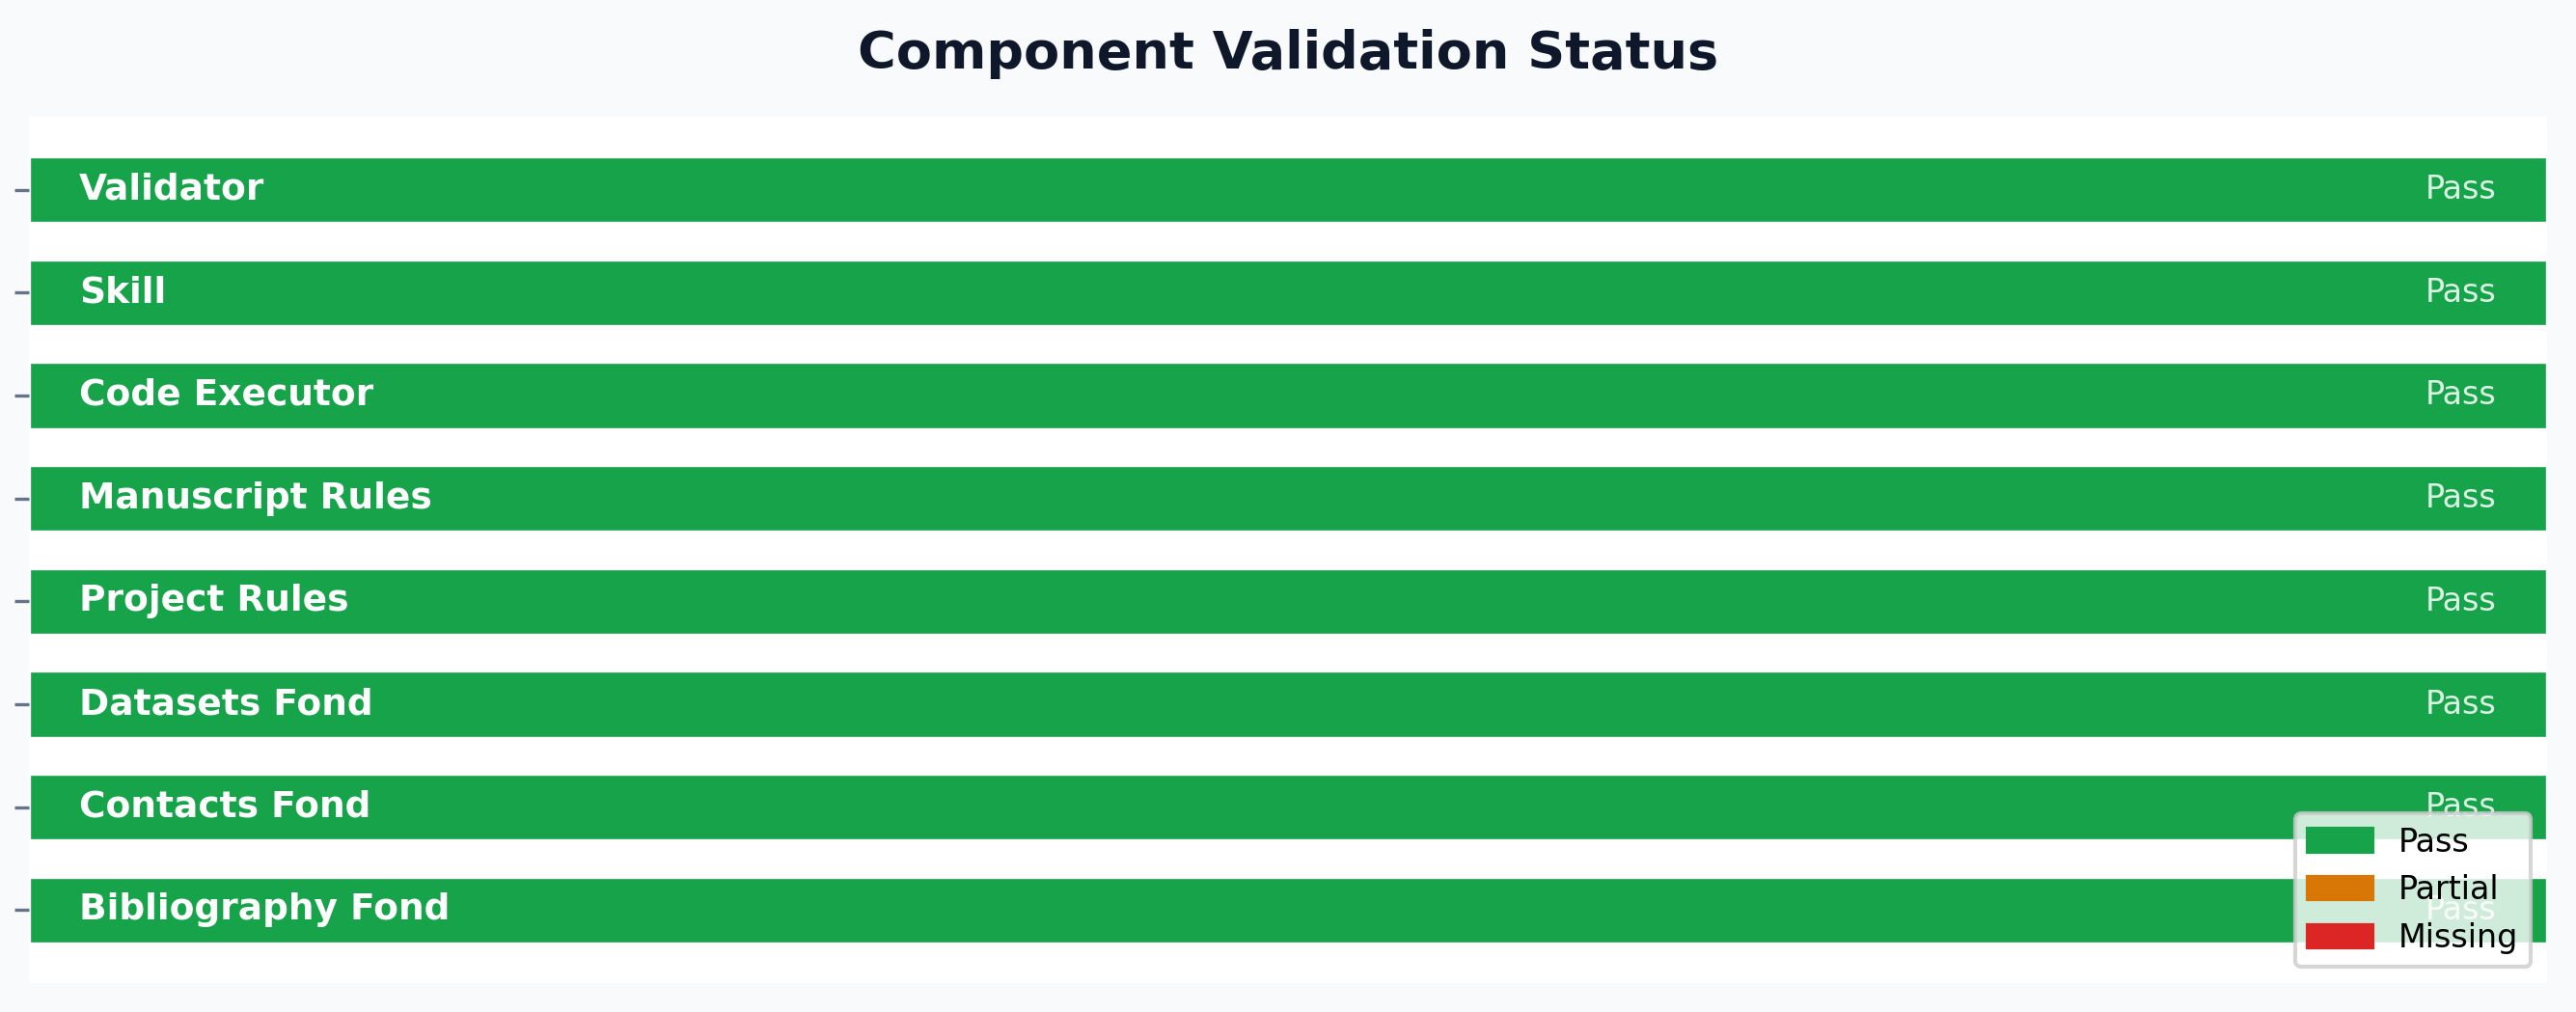
\includegraphics[width=0.85\linewidth,height=0.50\textheight,keepaspectratio,alt={Integration status dashboard showing per-resource validation results. Green indicates ok, amber indicates partial, red indicates missing.}]{../figures/status_dashboard.png}
\caption{Integration status dashboard showing per-resource validation
results. Green indicates ok, amber indicates partial, red indicates
missing.}\label{fig:pipeline}
\end{figure}

fig.~\ref{fig:pipelineflow} traces this sequence left to right: source
validation feeds the integration demo, whose summary feeds both the
manuscript-variable token file and the strong-rule semantic evaluator;
the figure-generation stage runs independently; and
\breaktt{z\_generate\_manuscript\_variables.py} --- invoked automatically
by the rendering pipeline immediately before the PDF render step --- is
what actually substitutes every \texttt{\{\{TOKEN\}\}} and writes the
resolved manuscript that pandoc consumes. fig.~\ref{fig:pipeline} shows
the corresponding per-component pass/partial/missing status from the
same run.

Each script imports all business logic from \texttt{src/} and stays free
of computation of its own --- the longest,
\breaktt{01\_validate\_sources.py} at 112 lines, is entirely CLI plumbing
(argument parsing, console formatting) around calls into
\breaktt{src/fonds\_reader.py}, \breaktt{src/rules\_applier.py}, and
\breaktt{src/tools\_invoker.py}. This thin-orchestrator pattern
\citep{Wilson2014best} ensures that all testable logic is in
\texttt{src/} at \texorpdfstring{\textgreater{}=}{>=} 90\% coverage, while the scripts themselves remain
readable without a dedicated test suite of their own.

\subsection{Resilience Design}\label{resilience-design}

The integration layer enforces resilience at three levels, corresponding
to the three failure modes a monorepo integration pipeline encounters:

\begin{enumerate}
\def\labelenumi{\arabic{enumi}.}
\item
  \textbf{Resource absence}: A fond, rule set, or tool directory may not
  yet exist if the resource was created by a parallel agent that has not
  yet completed. All three reader modules return \texttt{None} or empty
  collections in this case, and \breaktt{run\_integration\_demo()}
  reports the missing resource in the \texttt{summary} dict without
  raising.
\item
  \textbf{Schema malformation}: A manifest may be present but contain
  invalid YAML or missing required fields. Readers catch
  \texttt{yaml.YAMLError} and return a degraded result
  (\breaktt{status="partial"} in rule validation; \texttt{None} in fond
  reading) rather than propagating the parse error.
\item
  \textbf{Script absence}: A tool may declare entrypoints in its
  manifest that have not yet been created.
  \breaktt{validate\_tool\_scripts\_exist()} detects this at discovery
  time and returns \breaktt{status="partial"} with a list of missing
  script paths, so the pipeline can report the defect without attempting
  to invoke a non-existent script.
\end{enumerate}

\begin{figure}
\centering
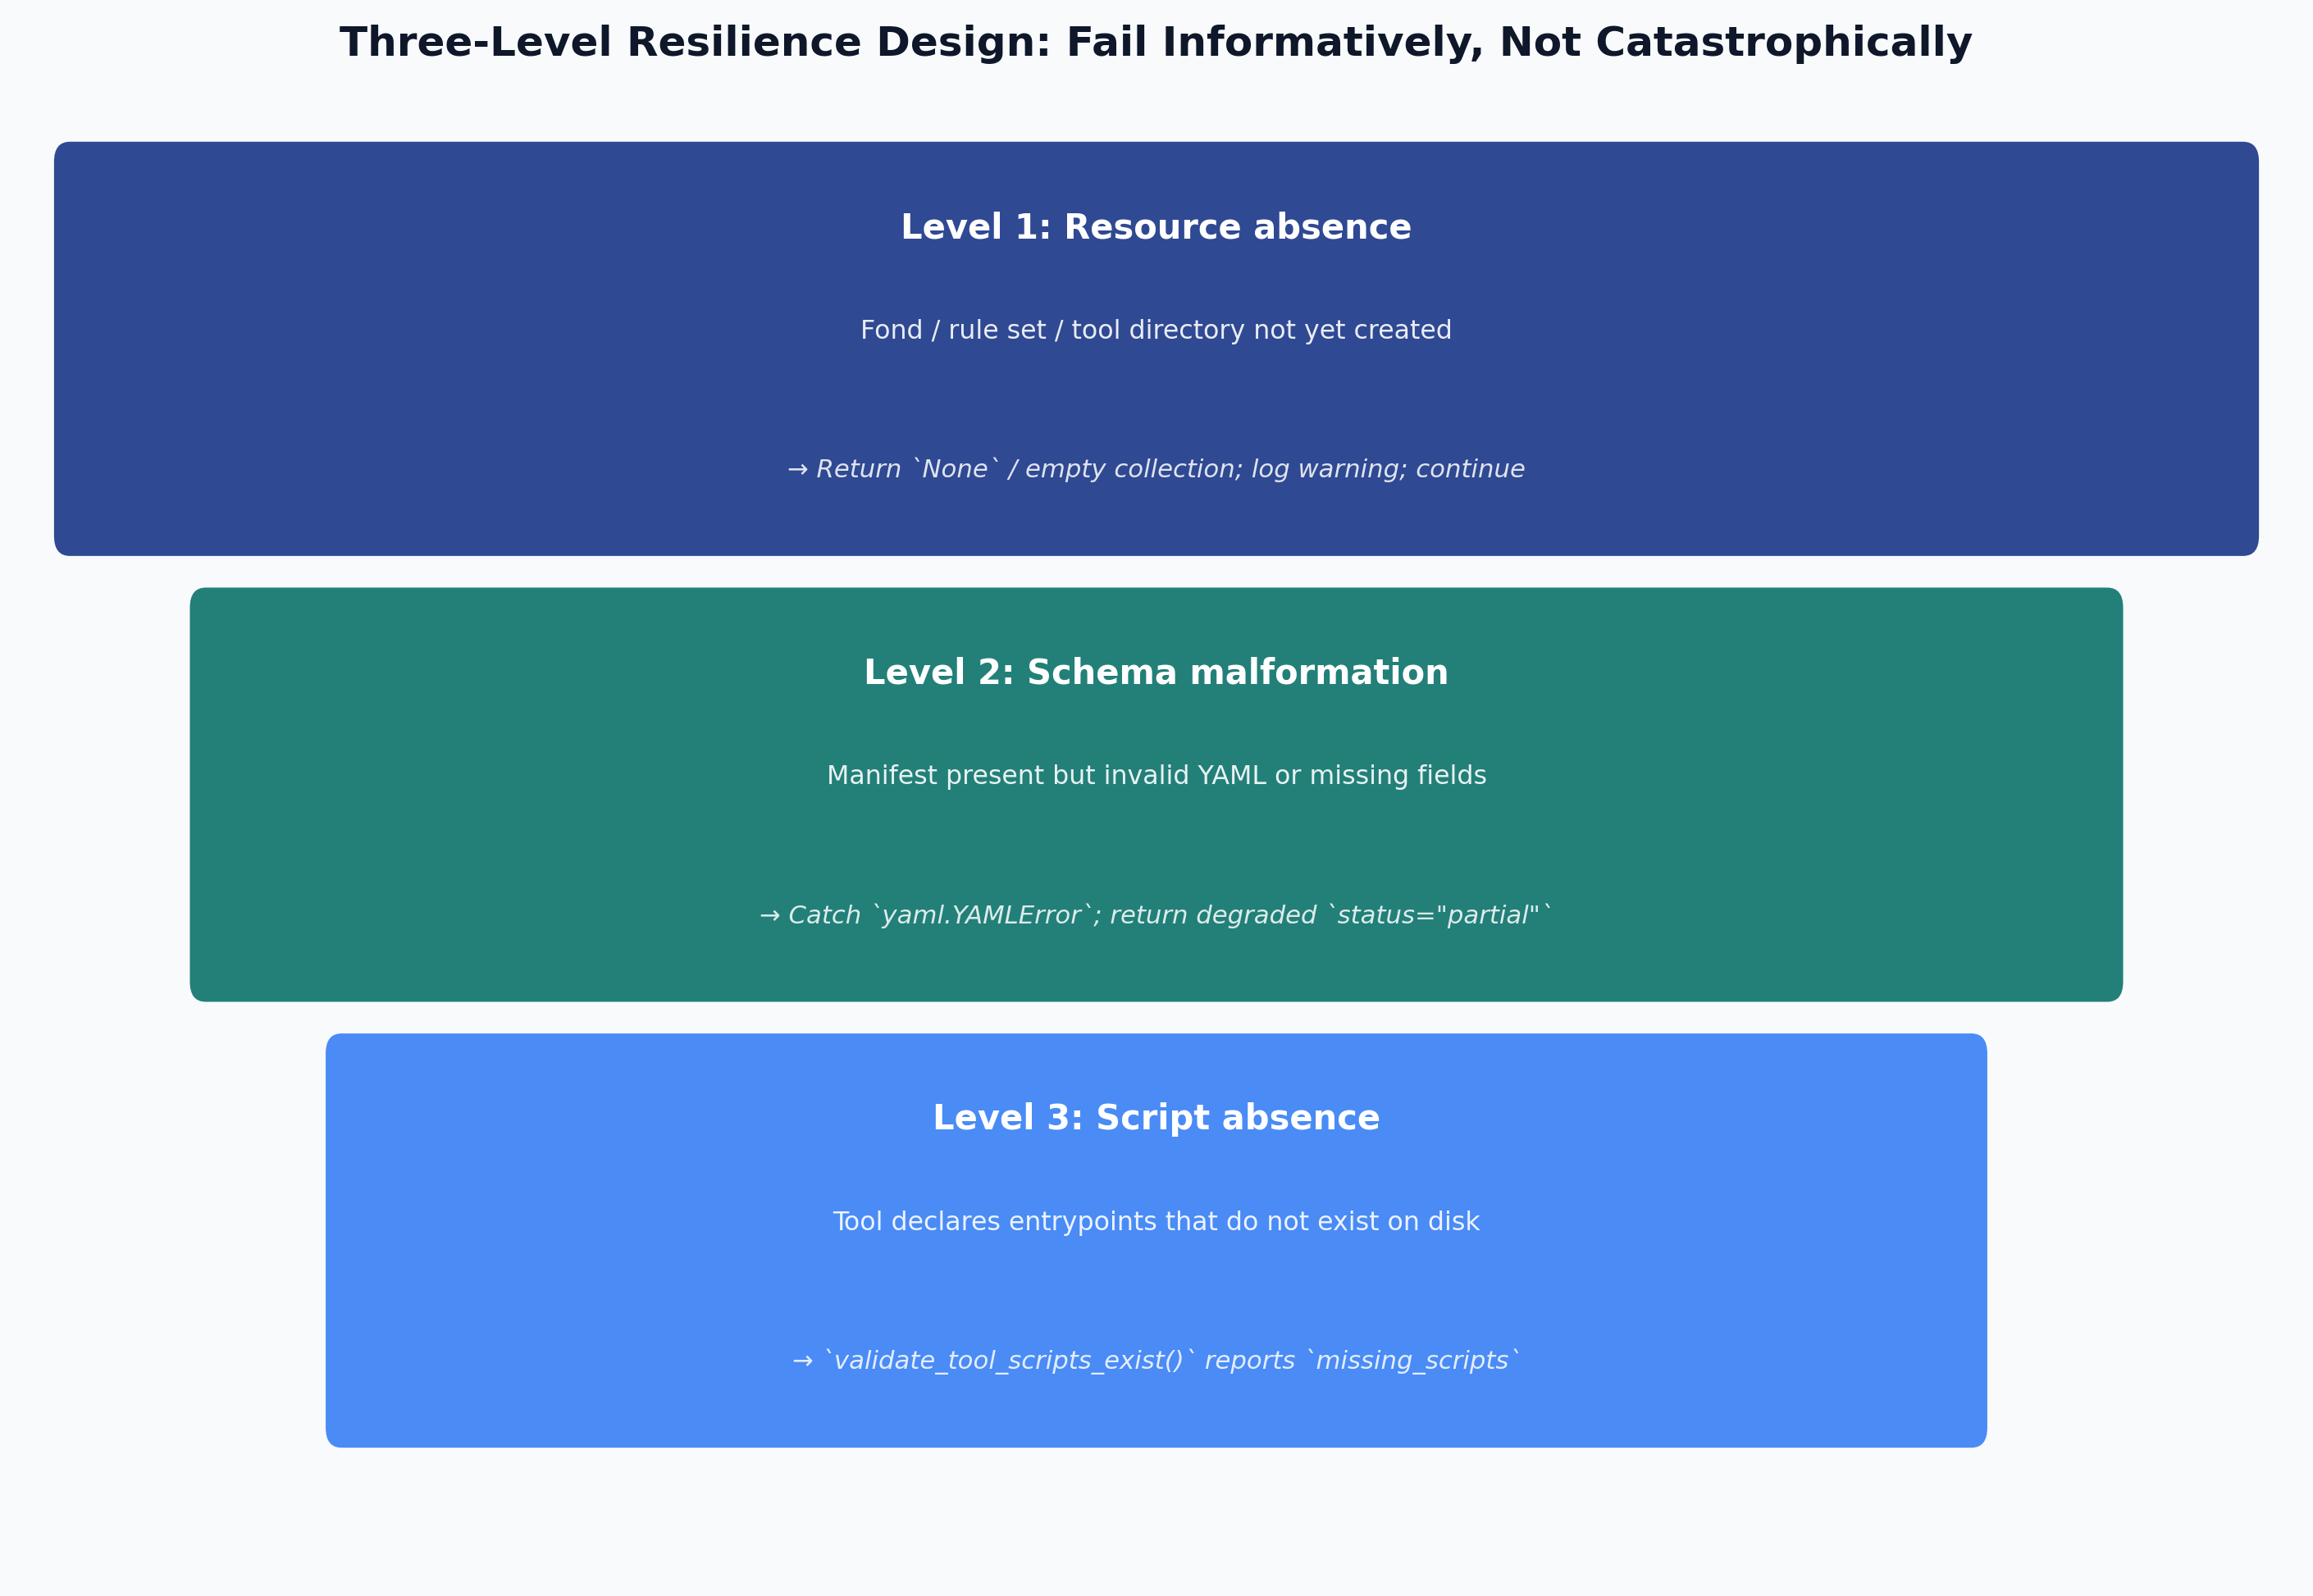
\includegraphics[width=0.85\linewidth,height=0.50\textheight,keepaspectratio,alt={The integration layer's three-level resilience design: resource absence, schema malformation, and script absence, each with its own graceful-degradation response.}]{../figures/resilience_layers.png}
\caption{The integration layer's three-level resilience design: resource
absence, schema malformation, and script absence, each with its own
graceful-degradation response.}\label{fig:resilience}
\end{figure}

This three-level resilience design reflects the principle that
shared-resource pipelines should fail \emph{informatively} rather than
\emph{catastrophically} --- surfacing the cause of incompleteness in
structured output that downstream consumers can act on
\citep{Taschuk2017ten}. fig.~\ref{fig:resilience} presents the three
levels as a single funnel: each level's failure mode and
graceful-degradation response, read top to bottom in the order a
pipeline run actually encounters them (resource discovery happens before
schema parsing, which happens before script-existence checks).

\subsection{Performance and Overhead}\label{performance-and-overhead}

The resilience design above trades a small, constant amount of I/O
overhead for the ability to degrade gracefully. Each reader performs at
most two filesystem existence checks (\breaktt{pathlib.Path.exists()})
before attempting a read, and every YAML parse uses
\breaktt{yaml.safe\_load()} rather than a schema-validating parser ---
the module deliberately performs \emph{structural} validation
(parseable, expected top-level keys present) and leaves deep
\emph{semantic} validation to the dedicated
\breaktt{strong\_rule\_evaluator} module (sec.~\ref{sec:rules}) rather
than paying that cost on every discovery call. In practice,
\breaktt{scripts/02\_run\_integration.py} completes in well under a
second on the exemplar's small fond/rule/tool counts; the design does
not attempt to optimise for repositories with thousands of fonds, since
the target use case is a curated, human-reviewed set of shared resources
rather than a large-scale data catalogue.

\subsection{Test Coverage}\label{test-coverage}

The eight \texttt{src/} modules --- \texttt{fonds\_reader},
\texttt{rules\_applier}, \texttt{tools\_invoker}, \texttt{integration},
\texttt{figures}, \breaktt{strong\_rule\_evaluator},
\breaktt{manuscript\_variables}, and \texttt{type\_defs} --- are covered
by tests across nine test files in \texttt{tests/}, including
property-based tests (\breaktt{test\_property\_based.py}) and
coverage-extras tests targeting previously-uncovered branches
(\breaktt{test\_coverage\_extras.py}). Tests use real file paths, real
YAML files, and real BibTeX content rather than mocks, ensuring that
coverage numbers reflect genuine code paths through the
resource-discovery logic. The current coverage report shows combined
line coverage comfortably above the project's 90\% floor;
\breaktt{strong\_rule\_evaluator.py}, the newest and most branch-heavy
module, has the most room for additional edge-case tests, while the
remaining seven modules are at or near 100\%. These exact test/coverage
counts drift as the suite grows --- treat the figures above as a
snapshot, not a frozen claim, and re-run
\breaktt{uv\ run\ pytest\ …\ -\/-cov-report=term} for the current
numbers. The \breaktt{tests/test\_integration.py} suite includes an
end-to-end test that calls \breaktt{run\_integration\_demo()} and asserts
that the \texttt{summary} dict contains the expected keys with
non-negative integer values --- a contract test that verifies the token
injection pipeline's data source.
\breaktt{tests/test\_manuscript\_variables.py} adds a negative control:
it monkeypatches \breaktt{run\_integration\_demo()}'s return value and
asserts the derived tokens actually change, proving the token-generation
function is live-wired to its source rather than emitting a hard-coded
constant.

\newpage

\section{Conclusion}\label{sec:conclusion}

\subsection{Summary}\label{summary}

This paper has presented \breaktt{template\_pools\_rules\_tools}, a
meta-project exemplar demonstrating how research software projects
embedded in a monorepo can integrate three categories of shared
resources --- data pools (fonds), governance rules, and executable tools
--- without tight coupling to any specific resource instance. The key
contributions are:

\begin{enumerate}
\def\labelenumi{\arabic{enumi}.}
\item
  \textbf{A four-module architecture} (\texttt{fonds\_reader},
  \texttt{rules\_applier}, \texttt{tools\_invoker},
  \texttt{integration}) that provides a canonical pattern for
  resource-aware project code in the template repository. Each module is
  independently testable and independently deployable.
\item
  \textbf{A typed manifest convention} (\texttt{fonds.yaml},
  \texttt{rules.yaml}, \texttt{tools.yaml}) that makes resource
  capabilities explicit and checkable at pipeline initialisation time,
  shifting failure detection from runtime to startup --- a significant
  improvement for reproducibility \citep{Wilson2014best}.
\item
  \textbf{A token injection pipeline} that links manuscript prose to
  integration runtime statistics through \texttt{\{\{UPPERCASE\_KEY\}\}}
  tokens, ensuring that quantitative claims in the manuscript are always
  generated by the pipeline rather than authored manually. In the
  current run this covered 3 fonds, 2 rule sets, 3 tools, and 8
  bibliography entries.
\item
  \textbf{A three-level resilience design} --- resource absence, schema
  malformation, and script absence --- that allows the pipeline to
  degrade gracefully and report failures informatively rather than
  crashing, consistent with best practices for robust research software
  \citep{Taschuk2017ten}.
\end{enumerate}

\subsection{Design Decisions
Revisited}\label{design-decisions-revisited}

Several design decisions deserve emphasis as lessons for future exemplar
authors:

\textbf{Repo-root-relative discovery} is non-negotiable in a forkable
monorepo. Any hard-coded absolute path or working-directory assumption
will fail when the repository is cloned to a different location. The
\texttt{pathlib.Path(\_\_file\_\_).resolve().parents{[}N{]}} idiom used
throughout \texttt{src/} ensures that discovery works from any working
directory.

\textbf{Graceful fallbacks over exceptions} is the correct trade-off for
a resource-consumption layer. The alternative --- raising
\breaktt{FileNotFoundError} when a fond is missing --- would make the
integration pipeline fragile to the ordering of parallel agent writes.
Returning \texttt{None} and logging a warning allows the pipeline to
produce a complete, if partial, result dict that downstream consumers
can reason about.

\textbf{Real-file tests over mocks} is required for a template exemplar.
Mocks can pass tests while the real discovery logic is silently broken.
Tests that use real file paths exercise the full path-resolution chain
and catch regressions that mocks would miss.

\textbf{Thin orchestration scripts} keep the scripts directory readable
and focus all testable logic in \texttt{src/}. A script that does more
than parse arguments, call a \texttt{src/} function, and write output is
accumulating business logic that belongs elsewhere.

\subsection{Limitations}\label{limitations}

This exemplar makes several deliberate simplifications that a reader
adopting the pattern should be aware of:

\begin{itemize}
\tightlist
\item
  \textbf{Structural, not semantic, validation by default.}
  \breaktt{validate\_against\_rules()} and \breaktt{discover\_tools()}
  confirm that manifests and rule files are parseable YAML with the
  expected top-level shape; they do not check that a fond's \emph{data}
  conforms to its declared schema, or that a tool's entrypoint script
  actually behaves according to its documented contract. Semantic
  constraint checking exists only for strong rules, via the separate
  \breaktt{strong\_rule\_evaluator} module (sec.~\ref{sec:rules}), and
  only for the constraint kinds that module implements:
  \breaktt{coverage\_threshold}, \breaktt{module\_structure},
  \texttt{section\_schema}, \breaktt{reference\_schema} (all four wired
  to a real strong-rule YAML file and exercised against this project's
  own live tree), plus \breaktt{manifest\_freshness} (evaluator logic
  implemented and unit-tested, deliberately not yet wired to a real rule
  file --- see Future Directions).
\item
  \textbf{No concurrency handling.} All readers assume a single-process,
  single-read invocation. If a parallel agent is actively writing a
  fond's \texttt{data/} file while another process reads it, the reader
  may observe a partially-written file and report a spurious parse error
  rather than a clean ``not yet available'' signal. The architecture
  tolerates \emph{absence} gracefully; it does not guarantee
  \emph{atomicity} against concurrent writers.
\item
  \textbf{Small-scale assumption.} As discussed in
  sec.~\ref{sec:integration}'s Performance and Overhead subsection, the
  design is tuned for a curated, human-reviewed set of resources
  (single-digit to low-double-digit counts per category), not a resource
  catalogue at data-lake scale.
\item
  \textbf{English-language, code-review-oriented soft rules.} Soft rules
  are Markdown prose intended for human reviewers and AI coding agents;
  they are not evaluated by any automated tool in this exemplar, unlike
  strong rules. A project that wants soft-rule compliance checked
  automatically would need to promote the relevant guideline to a strong
  rule with a corresponding evaluator function.
\item
  \textbf{\breaktt{strong\_rule\_evaluator.py} had the thinnest test
  coverage of any \texttt{src/} module, historically.} As measured in an
  earlier coverage run this session, it required more negative-control
  tests (malformed rule files, real violations, type-mismatched context
  values) than the other seven modules, concentrated in its
  \texttt{section\_schema}, \breaktt{reference\_schema}, and
  \breaktt{module\_structure} evaluators and its context loader. That gap
  has since been closed with real negative-control fixtures --- run
  \breaktt{uv\ run\ pytest\ …\ -\/-cov-report=term-missing} for the
  current per-module breakdown, since these numbers, like the ones
  above, drift as the suite grows.
\end{itemize}

\textbf{The no-concurrency-handling limitation above is not merely
theoretical}: this exemplar is itself designed to be populated by
parallel agents authoring \texttt{fonds/}, \texttt{rules/}, and
\texttt{tools/} concurrently, which is precisely the scenario where a
torn read is most likely. Adopters running this pattern in a genuinely
concurrent write environment should add file locking or an atomic-rename
write pattern at the resource-authoring layer --- this exemplar
deliberately does not, to keep the reader-side code minimal.

\subsection{Future Directions}\label{future-directions}

The three-layer architecture described here is deliberately extensible.
The most natural extension is a fourth resource category:
\textbf{models}
(\texttt{models/\textless{}scope\textgreater{}/\textless{}name\textgreater{}/})
for pre-trained machine learning models and their inference scripts. The
pattern would follow exactly the same manifest-and-reader design, with
\texttt{models.yaml} declaring type, version, and entrypoints, and a
\texttt{models\_loader} module providing \breaktt{discover\_models()} and
\breaktt{validate\_model\_files\_exist()}. Adding this layer to
\breaktt{template\_pools\_rules\_tools} would require only a new reader
module and a new section in the integration orchestrator --- the
existing architecture places no constraints on the number of resource
categories.

A second direction, \textbf{cross-fond validation}, is now implemented:
\breaktt{src/integration.py::check\_bibliography\_overlap()} compares
this manuscript's own cite keys against the
\breaktt{template\_bibliography} fond's curated set and reports
\texttt{overlap}, \texttt{project\_only}, and \texttt{fond\_only}
counts. It deliberately does \emph{not} assert full containment in
either direction --- this manuscript legitimately cites
software-engineering sources the fond does not curate, and the fond
legitimately curates machine-learning sources this manuscript does not
cite. Run
\breaktt{uv\ run\ python\ -c\ "from\ src.integration\ import\ check\_bibliography\_overlap;\ import\ json;\ print(json.dumps(check\_bibliography\_overlap(),\ indent=2))"}
from the project root to see the current overlap.

A third direction, suggested directly by the Limitations above, was
extending \breaktt{strong\_rule\_evaluator} with additional rule kinds
beyond the original four. The \breaktt{manifest\_freshness} kind ---
flagging a fond whose \texttt{version} field has not been bumped despite
its \texttt{data/} files changing more recently than its manifest --- is
now implemented:
\breaktt{src/strong\_rule\_evaluator.py::\_evaluate\_manifest\_freshness()}
is a fifth dispatch entry, unit-tested against synthetic rule dicts
(\breaktt{tests/test\_strong\_rule\_evaluator.py}). It is deliberately
\textbf{not} yet wired to a real strong-rule YAML file: doing so would
mean adding a file under the shared
\breaktt{rules/templates/template\_project\_rules/strong/} or
\breaktt{rules/templates/template\_manuscript\_rules/strong/} directory,
which this project's own read-only contract against \texttt{fonds/},
\texttt{rules/}, and \texttt{tools/} reserves for an explicit decision
rather than a routine content edit. The evaluator's logic is proven
correct against synthetic input; proving it against a real fond's real
manifest and data-file timestamps is the natural next step, pending that
decision.

The exemplar is ready to fork. A project team wishing to adopt this
architecture need only copy the relevant \texttt{src/} modules (the
three readers plus \texttt{integration.py} are the minimum;
\breaktt{strong\_rule\_evaluator.py} and \texttt{figures.py} are optional
extensions), update the resource directory paths in each reader, and
replace the exemplar fond/rules/tool names with their own.



\clearpage

\bibliography{references}
\end{document}
